% IEEEAerospace2012.cls requires the following packages: times, rawfonts, oldfont, geometry
\documentclass[twocolumn,letterpaper]{IEEEAerospaceCLS}  % only supports two-column, letterpaper format

% The next line gives some packages you may find useful for your paper--these are not required though.
%\usepackage[]{graphicx,float,latexsym,amssymb,amsfonts,amsmath,amstext,times,psfig}
% NOTE: The .cls fil is now compatible with amsmath!!!
% \newcommand\hmmax{1}
% \newcommand\bmmax{1}
% \usepackage{bm}
\usepackage{color}
\usepackage{float}
\usepackage{amsthm}
\usepackage{xcolor}
\usepackage{amsmath}
\usepackage{amssymb}
% \usepackage{bigints}
\usepackage{comment}
\usepackage{environ}
\usepackage{siunitx}
\usepackage{wrapfig}
\usepackage{amsfonts}
\usepackage{etoolbox}
\usepackage{fancyhdr}
\usepackage{graphicx}
\usepackage{hyperref}
\usepackage{lettrine}
\usepackage{mdframed}
\usepackage{multirow}
% \usepackage{nathtools}
\usepackage{subcaption}
% \usepackage{algorithm}
\usepackage{algorithm2e}
% \usepackage[noend]{algpseudocode}
\usepackage{indentfirst}
\usepackage[version=4]{mhchem}
\usepackage{longtable}
\usepackage{tabularx}
\usepackage[style=ieee]{biblatex}
\usepackage{dblfloatfix}
\addbibresource{bibliography.bib}

% \usepackage{fontspec}
% \setmathfont{TeX Gyre Pagella}

\setlength\LTleft{0pt}
\newcommand{\ignore}[1]{}  % {} empty inside = %% comment
% \DeclareMathAlphabet{\mathbb}{U}{bbold}{m}{n}
\newtheorem{theorem}{Theorem}[section]
\newtheorem{corollary}{Corollary}[theorem]
\newtheorem{lemma}[theorem]{Lemma}

\begin{document}

\title{Capturing Tumbling Objects in Orbit\\with Adaptive Tube Model Predictive Control}

\author{%
Aaron John-Sabu\\ 
Graduate Student\\
Department of Mechanical and Aerospace Engineering\\
The University of California, Los Angeles (UCLA)\\
Los Angeles, CA 90095\\
aaronjs@g.ucla.edu
\and 
Brett T. Lopez\\
Asst. Professor\\
Department of Mechanical and Aerospace Engineering\\
The University of California, Los Angeles (UCLA)\\
Los Angeles, CA 90095\\
btlopez@ucla.edu
\thanks{\footnotesize 979-8-3503-0462-6/24/$\$31.00$ \copyright2024 IEEE}}

\maketitle

\thispagestyle{plain}
\pagestyle{plain}

\maketitle

\thispagestyle{plain}
\pagestyle{plain}

\begin{abstract}
There is a growing need for sophisticated rendezvous and docking guidance algorithms capable of capturing tumbling, noncooperative objects, e.g., space debris, before they collide with other satellites.
In this paper, we address the problem of safely capturing and stabilizing tumbling objects despite the presence of parametric variations in the dynamics model.
This capability entails sending a specialized spacecraft (referred to as the chaser) that attaches to a tumbling object (referred to as the target) to stabilize or deorbit the noncooperative asset.
While rendezvous and docking with cooperative objects has been possible for several decades, advanced strategies for tumbling objects that account for uncertainties in the model parameters of either the chaser or target are still under development.
We propose the use of adaptive dynamic tube model predictive control (ADTMPC) for trajectory planning of the chaser for rendezvous and docking with the target.
Traditionally, the presence of model uncertainty requires the use of robust guidance techniques that are often conservative, leading to suboptimal performance.
The main advantage of our approach is the ability to safely update the prediction model online -- leading to less conservative trajectories and behaviors -- without violating safety constraints that include time-varying collision constraints and other standard state or control constraints.
The approach relies on computing a suitable robust tracking controller offline and combining it with a set membership identification algorithm that identifies the feasible set of parameters online rather than a single point estimate.
Under mild assumptions, we guarantee the system will always satisfy the specified constraints even as the model is changing online.
Moreover, our approach can incorporate predictions of how the closed-loop trajectory tracking performance will vary with the designed trajectory.
This property, in essence, can be used to inform the guidance algorithm on which maneuvers can be executed without exciting the uncertain system dynamics.
For the docking phase, we also propose an optimization-based procedure for computing the optimal docking position of the chaser on the target and the optimal application of propulsion to detumble the target.
We first demonstrate our approach for a single chaser-target scenario where drag, inertial parameters, and orbit parameters are uncertain.
A multi-chaser strategy is also explored.
\end{abstract}
\tableofcontents
\setcounter{secnumdepth}{3}
\section{Nomenclature}
{\renewcommand\arraystretch{1.0}
\noindent\begin{longtable*}{@{}l @{\quad=\quad} l@{}}
$\mathsf{e}$            & eccentricity \\
$\alpha$                & drag constant of the target\\
$\beta$                 & drag constant of the chaser\\
$t$                     & time elapsed since perigee\\
$\theta$                & true anomaly elapsed since perigee\\
$\boldsymbol{r}$        & position of the chaser\\
$\boldsymbol{u}$        & control input of the chaser\\
$\boldsymbol{\theta}$   & angular position of the target\\
$\boldsymbol{\omega}$   & angular velocity of the target\\
\end{longtable*}}
%%%%%%%%%%%%%%%%%%%%%%%%%%%%%%%%%%%%%%
\section{Introduction}
%%%%%%%%%%%%%%%%%%%%%%%%%%%%%%%%%%%%%%
\lettrine{S}{ince} the creation of human-made orbital debris following the launch of Sputnik 1 in 1957, the first piece being the rocket stage that launched the artificial satellite and the second being the satellite itself, the presence of debris in orbit has increased dramatically.
Currently, about 27,000 officially cataloged objects, many of them non-functional and hence non-cooperative, are still in orbit and most of them are $10$ cm and larger. % https://www.nasa.gov/mission_pages/station/news/orbital_debris.html
Such non-cooperative systems in orbit lead to the threat of collision, potentially leading to the Kessler syndrome, the scenario where a sufficiently large collision of spacecraft could lead to a cascade effect and probably even make some low Earth orbits unusable for long-term use.
These collisions have involved operational satellites in the past such as the collision of Iridium 33, a communications satellite, with Cosmos 2251, an inactive Russian military communications satellite in 2009.
Our research is inspired by the need to control and deflect tumbling non-cooperative objects in orbit so as to avoid the risk of collisions with more vital orbiting systems such as functional satellites and space stations.

\cite{albee2021robust} presents techniques on rendezvous and control of such tumbling objects using a single spacecraft agent.
Although this has been conceptualized using single-agent systems, larger tumbling objects (hereon also referred to as 'targets') require multiple agents (hereon also referred to as 'chasers') to be brought to a standstill.
Furthermore, the paper assumes the accurate calculation of potentially unknown inertial and orbital parameters which may not always be true.
% In order to solve the problem of autonomous multi-agent interaction and deflection of uncooperative and adversarial objects in orbit, we consider @@@
As a result, we reconsider this problem considering the estimation of unknown parameters and the potential for extension to multiple chasers.

Previous research on on-orbit servicing has dealt with a similar problem where the chaser is attached to the target to perform repairs and similar operations \cite{nakka2022information,battistini2022iterative}.
However, such research assumes the cooperation of the target in terms of sharing information.
This is not the case with non-cooperative space debris that is inert and shut down in orbit.
We also draw motivation from previous literature on on-orbit inspection, especially using multiple chasers \cite{long2007orbit}.
However, this research delves into interaction with the target beyond inspection in order to stop the tumble of the target.

Chaser-target interaction can be made possible using several techniques.
These include the use of tethers by the chaser to attach onto a target that is at a distance \cite{zhang2019trajectory,olivieri2020test}.
While it is possible for an operational satellite or spacecraft to be either partially cooperative (via communication of target characteristics and dynamics) in the case of the on-orbit servicing problem, much of space debris is `non-cooperative and passive' \cite{albee2021robust}.
In addition, the tumble of the target would make it seemingly impossible to attach a free-flying tether at a specific location on the target.
Previous research \cite{park2017nonlinear} has dealt with this by instead proposing techniques to perform rendezvous and docking with the target.
Although this is a feasible solution, the possibility for collisions is very likely.
As a result, our research proposes rendezvous and docking along with the simultaneous estimation of unknown target parameters and the incorporation of robust techniques to prevent collisions.
\section{Relevant Knowledge and Problem Formulation}
\label{sec:relevant-knowledge}
%% Describe relevant orbital parameters - eccentricity, true anomaly, the relation between true anomaly and time, and drag coefficients
The translational dynamics of the chaser are considered to be in the local-vertical-local-horizontal (LVLH) frame of reference of the target.
As depicted in Figure \ref{fig:lvlh_frame}, this reference frame is centered at the center of mass of the target and fixed with respect to the orbit with its Y-axis pointing radially into the center of the Earth, the X-axis pointing opposite to the direction of the velocity of the target spacecraft, and the Z axis pointing along the angular momentum vector of the target, hence completing a right-handed system.
\begin{figure}[htb]
    \centering
    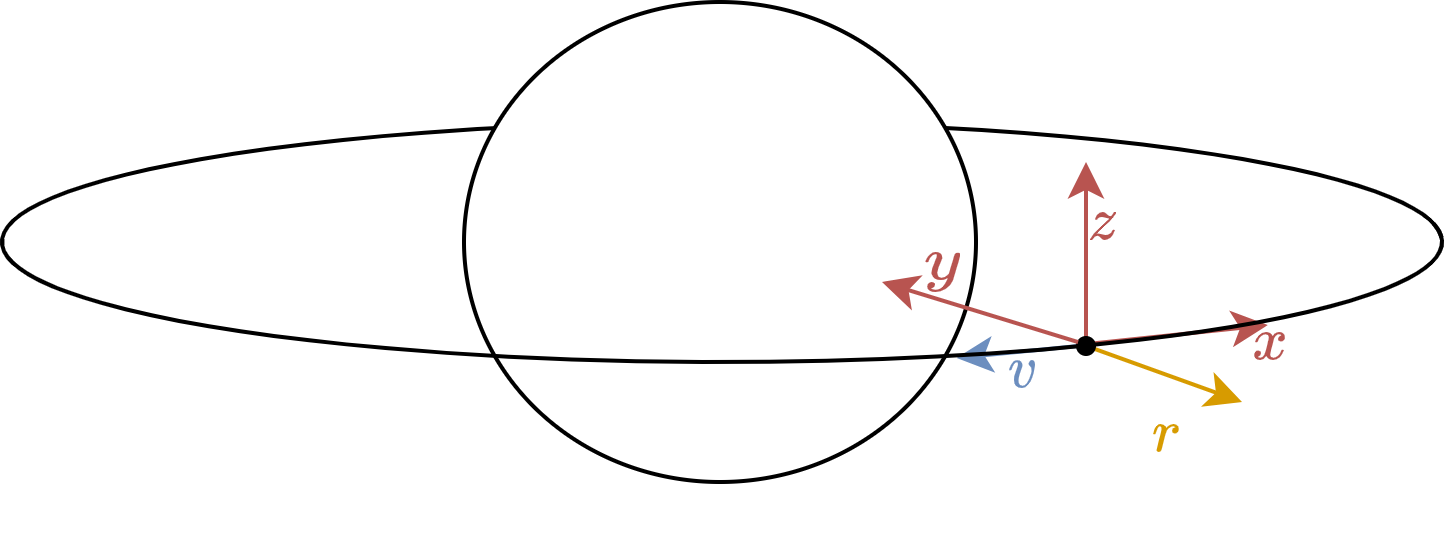
\includegraphics[width=0.9\linewidth]{assets/lvlh_frame.png}
    \caption{Local-Vertical-Local-Horizontal (LVLH) Frame of Reference of the Target}
    \label{fig:lvlh_frame}
\end{figure}
If we assume the orbits of the target and the chaser to be circular, within close proximity to the target, the translational dynamics of the chaser follow the Clohessy-Wiltshire-Hill (CWH) equations (refer to Appendix \ref{app:cwh-equations}).
However, in this paper, we generalize the problem to targets that may be in elliptical orbits around the Earth.
Appendix \ref{app:ellp-undrag} describes the dynamics of relative motion in an elliptical orbit where the chaser and the target may have unequal drag constants.
As considered in the paper, we assume an inverse law, $g(R)=1/R$, to model the variation in atmospheric density.
However, we realize that this inverse law does not perfectly represent the scale of the trend of atmospheric density \cite{emmert2021nrlmsis}.
As a result, we consider the corresponding ratio in variation into the drag constants $\alpha$ (of the target) and $\beta$ (of the chaser).
Such a system considers the true anomaly $\theta$ of the orbit as the independent variable, hence giving the following dynamical equations:
\begin{subequations}\label{second:main}
\begin{align}
    \boldsymbol{r}'(\theta)&=A(\theta,\theta_0)\boldsymbol{r}(\theta)+B\boldsymbol{u}(\theta)+\boldsymbol{d}(\theta, \theta_0)\tag{\ref{second:main}}\\
    \text{where }\boldsymbol{r}(\theta)&=\begin{bmatrix}
    x(\theta),y(\theta),z(\theta),x'(\theta),y'(\theta),z'(\theta)
    \end{bmatrix}^T,\\
    \boldsymbol{u}(\theta)&=\begin{bmatrix}
    u_x(\theta),u_y(\theta),u_z(\theta)
    \end{bmatrix}^T
\end{align}
\end{subequations}
As a result, we will consider true anomaly to be the primary independent variable throughout this paper.
The relation between the true anomaly of the target and the time lapsed since periapsis $t=t_{\text{curr}}-t_p$ is given as:
\begin{subequations}
\begin{align}
    M&=M_0+2\pi\frac{t}{T}\\
    M&=E-{\mathsf{e}}\sin(E)\\
    \theta&=E+2\arctan\left(\frac{\beta\sin(E)}{1-\beta\cos(E)}\right)\\
    \beta&=\frac{{\mathsf{e}}}{1+\sqrt{1-{\mathsf{e}}^2}}
\end{align}
\end{subequations}
where $M$ is the mean anomaly of the target, $E$ is the eccentric anomaly of the target, and ${\mathsf{e}}$ is the eccentricity of the orbit of the target.
Hence, the true anomaly of the orbit can be numerically computed from time and time can be analytically computed from true anomaly.\\
% To follow consistent nomenclature, we use $\theta$ in this paper to represent the true anomaly of the chaser-target system and $\boldsymbol{\theta}$ to represent the angular position of the target.\\
Based on the given information above and the need for reliable solutions to the detumbling problem in orbit, we propose the application of adaptive dynamic tube model predictive control (ADTMPC) to facilitate chaser trajectory planning for rendezvous and docking.
Section \ref{sec:chaser_ampc} deals with the basic trajectory optimization problem followed by the estimation of unknown parameters using adaptive control techniques.
Section \ref{sec:constraints} elaborates on the constraints and bounds involved in this problem. 
This is followed by an explanation of the effects of using dynamic tubes to avoid constraint violation in Section \ref{sec:dynamic-tube}.
Section \ref{sec:multi-agent} proposes techniques to expand this problem using multiple chasers.
The chaser, following its attachment onto the target, needs to exert torque on the target to stop detumbling.
This is discussed in Section \ref{sec:target-deflection}.
We also demonstrate the effectiveness of using ADTMPC over other techniques that do not include elements of this algorithm.
Finally, the appendices provide more information on the dynamics of the chaser for a simplistic (circular orbit with no drag) scenario followed by a more realistic (elliptical orbit with quadratic drag) one.
\section{Adaptive Model Predictive Control for Trajectory Planning} \label{sec:chaser_ampc}
% Following the determination and consensus of the goal states of all chasers, they individually plan trajectories from their start positions to the goal positions. Due to the uncertainty of orbital dynamics due to factors such as the potentially elliptical nature of the orbit, electromagnetic fluctuations, and solar radiation, we propose the application of model predictive control to plan the trajectory of the chaser for rendezvous (initial approach) with the target.
The problem of rendezvous deals with the approach of the chaser from a farther location to a location close to the target.
Due to the uncertainty of orbital dynamics as a result of factors such as the potentially elliptical nature of the orbit, electromagnetic fluctuations, and solar radiation, we propose the application of adaptive model predictive control to plan the trajectory of the chaser for rendezvous (initial approach) with the target.
The uncertainty caused by the elliptical nature of the target's orbit can be traced back to the eccentricity of the orbit.
This orbit can be modeled using the Tshauner-Hempel equations \cite{yamanaka2002new,sinclair2015geometric}
We also consider the effect of non-conservative forces such as (quadratic) atmospheric drag \cite{carter2002clohessy} on the target and the chaser which can be represented using the drag constants of the spacecraft.
These quantities can be formulated as unknown parameters in the problem and learned over time based on the error in the estimated state of the chaser, $\hat{\boldsymbol{r}}$, with respect to its actual state, $\boldsymbol{r}$.
For this purpose, the chaser implements adaptive model predictive control (AMPC) wherein it plans trajectories and updates the calculated trajectory at regular intervals while also updating the estimates for the unknown quantities.

\subsection{Trajectory Planning} \label{ssec:rendezvous-traj-planning}
The rendezvous trajectory planning problem involves generating trajectories such that the goal state is on a sphere around the target; i.e., at a fixed predetermined distance from the target.
% (The sphere can be replaced by any scaled convex shape that completely contains the target as explained later in Section \ref{sec:obs_sphere}.)
The chaser may require one or more intermediate goal locations to observe the target and estimate its physical and inertial properties.
This process of goal radius calculation is repeated for closer rendezvous until the distance between the target and the chaser is sufficiently small enough to initiate docking.
As a result, the trajectory planning problem for rendezvous can be formulated as the following optimization problem:
\begin{subequations}\label{first:main}
\begin{alignat}{2}
    \min_{\boldsymbol{r}, \boldsymbol{u}}\ &J(\boldsymbol{r}(\theta),\boldsymbol{u}(\theta))&&=h(\boldsymbol{r}(\theta_f))\notag\\
    & &&+\int_{\theta_0}^{\theta_f} \left((\boldsymbol{r}(\theta)-\boldsymbol{r}_f)^TQ(\boldsymbol{r}(\theta)-\boldsymbol{r}_f)\right.\notag\\
    & &&\qquad\quad\left.+\boldsymbol{u}(\theta)^TR\boldsymbol{u}(\theta)\right)d\theta\tag{\ref{first:main}}\\
    \textrm{s.t. } & \boldsymbol{r}'(\theta)=A(\theta)\boldsymbol{r}(&&\theta)+B(\theta)\boldsymbol{u}(\theta)+\boldsymbol{d}(\theta),\ \ \boldsymbol{u}\in{\mathbb{U}}\\
    & \boldsymbol{r}(\theta_0)=\boldsymbol{r}_0,&&\\
    &\boldsymbol{r}(\theta)\in{\mathcal{C}}_R\ &&\forall\ \theta\in[\theta_0,\theta_f]\label{eqn:radial-limit-constraint}
\end{alignat}
\end{subequations}
where the system dynamics are given by the extended Tshauner-Hempel equations (explained in Appendix \ref{app:ellp-undrag}), $\boldsymbol{r}_0$ represents the starting point of the chaser, final state cost function $h(\boldsymbol{r}(\theta_f))$ is minimized to move closer to the target, and ${\mathbb{U}}$ represents the range of permissible control input of the chaser.
The additional non-convex 'radial-limit' constraint in Equation \ref{eqn:radial-limit-constraint} ensures that the chaser remains outside all possible locations of the target, hence avoiding collisions.
This is further explained in Section \ref{sec:rendezvous-collision-constraints}.\\
The problem of docking is identical in structure and dynamics to rendezvous.
However, in order to make physical contact feasible, the collision constraints are modified with consideration of the physical (such as the angular velocity) and inertial (such as the moment of inertia) parameters of the target.
As a result, the 'radial-limit' constraint is replaced by a 'target-limit' constraint ${\mathcal{C}}_D$ as explained in Section \ref{sec:time-varying-collision-constraints}.
Moreover, the final state cost function is made stricter to achieve docking with the target.

\subsection{Estimation of Inertial and Angular Parameters of the Target}
\label{sec:target-estimation}
We will observe in Section \ref{sec:time-varying-final-state-constraint} that, at any given time, the final state of the chaser; i.e., the docking position is determined by the current angular position of the target and a predetermined point that is fixed in the body frame of the target.
This point is calculated via optimization of control input as explained in Section \ref{sec:target-deflection}.
(For the sake of this discussion, we consider all angles to be described using Tait-Bryan rotations.)
As a result, it is vital to estimate the inertial and angular parameters of the target.
We do not directly address this problem in this paper.
On the other hand, we encourage the reader to refer to \cite{setterfield2018inertial} on the estimation of such parameters using polhode analysis and similar techniques.\\
However, as observed later in Sections \ref{sec:rendezvous-collision-constraints} and \ref{sec:time-varying-collision-constraints}, although not required for the rendezvous collision constraints, the collision constraint in the docking problem also requires an accurate parameter estimation of the target.
This depends subsequently on the unknown parameters discussed earlier - the eccentricity of the orbit and the drag constant of the target.
In order to estimate these quantities, we introduce adaptive control using set membership identification (SMID).
As explained in \cite{morozov2020performance}, recursive feasibility (meaning that the problem remains feasible for all time) of the MPC operation requires that system uncertainty is monotonically non-increasing throughout adaptation.
This is achieved in our implementation of adaptive control using SMID since the feasible solution set (FSS) shrinks monotonically over time (Refer to Step 2 of Algorithm \ref{alg:smid}).
The progression of estimation using this SMID implementation is demonstrated in Figure \ref{fig:smid}.
\begin{algorithm}
    \textbf{Step 1:} \underline{Generate a Feasible Solution Set (FSS)}\\
    \hspace{2em}\textbf{Step 1a: }$\underline{{\mathsf{e}}}_{est} = \text{\textbf{minimize}}\ {\mathsf{e}}$\\
    \hspace{2em}\textbf{Step 1b: }$      \overline{{\mathsf{e}}}_{est} = \text{\textbf{maximize}}\ {\mathsf{e}}$\\
    \hspace{2em}\textbf{Step 1c: }$\underline{\alpha}_{est}   = \text{\textbf{minimize}}\ \alpha$\\
    \hspace{2em}\textbf{Step 1d: }$      \overline{\alpha}_{est}   = \text{\textbf{maximize}}\ \alpha$\\
    \hspace{4em}such that $\boldsymbol{r}'(\theta)=A(\theta)\boldsymbol{r}+B(\theta)u(\theta)+d(\theta)$\\
    \hspace{5em}$\boldsymbol{r}^P(\theta_0)=\boldsymbol{w}(\theta_0)$, $||\boldsymbol{r}^P(\theta_f)-\boldsymbol{w}(\theta_f)||\leq D$\\
    \hspace{5em}${\mathsf{e}}\in{\mathcal{E}}$, $\alpha  \in{\mathcal{A}}$\\
    \textbf{Step 2:} \underline{Define the new FSS}\\
    \hspace{3em}${\mathcal{E}}_{new}={\mathcal{E}}\cap[\underline{{\mathsf{e}}}_{est}, \overline{{\mathsf{e}}}_{est}]$\\
    \hspace{3em}${\mathcal{A}}_{new}={\mathcal{A}}\cap[\underline{\alpha}_{est},   \overline{\alpha}_{est}]$\\
    \textbf{Step 3:} \underline{Verify the new FSS}\\
    \hspace{3em}attempt to generate $x(t_f)$\\
    \hspace{4em}such that $\boldsymbol{r}'(\theta)=A(\theta)\boldsymbol{r}+B(\theta)u(\theta)+d(\theta)$\\
    \hspace{5em}$\boldsymbol{r}^P(\theta_0)=\boldsymbol{w}(\theta_0)$, $\boldsymbol{r}^P(\theta_f)\approx \boldsymbol{w}(\theta_f)$\\
    \hspace{5em}${\mathsf{e}}\in{\mathcal{E}}_{new}$, $\alpha  \in{\mathcal{A}}_{new}$\\
    \textbf{Step 4:} \underline{Compare and Update the FSS}\\
    \hspace{3em}if Step 3 works:\\
    \hspace{5em}${\mathcal{E}}\leftarrow{\mathcal{E}}_{new}$\\
    \hspace{5em}${\mathcal{A}}\leftarrow{\mathcal{A}}_{new}$\\
    \hspace{3em}else:\\
    \hspace{5em}do nothing\\
    \textbf{Step 5:} \underline{Update Data Range for Adaptation}\\
    \hspace{3em}consider new data by updating $\theta_0$ and $\theta_f$ as:\\
    \hspace{5em}$\Delta\theta = \theta_f - \theta_0$\\
    \hspace{5em}$\theta_0 \leftarrow \theta_f$\\
    \hspace{5em}$\theta_f \leftarrow \theta_f + \Delta \theta$\\~\\
    \caption{Implementation of the \textbf{Set Membership Identification (SMID) algorithm} over several MPC iterations}
    \label{alg:smid}
\end{algorithm}
\begin{figure}[htb]
    \centering
    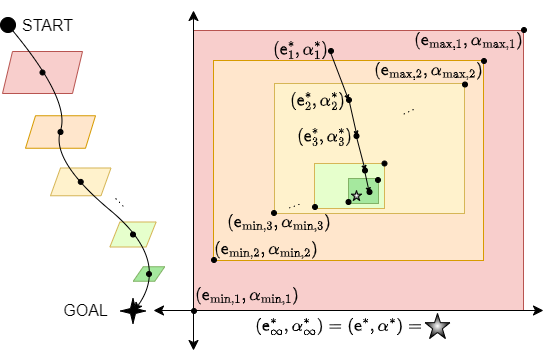
\includegraphics[width=0.98\linewidth]{assets/smid.png}
    \caption{Implementation of the Set Membership Identification (SMID) Algorithm}
    \label{fig:smid}
\end{figure}
We draw motivation from the idea of MSAC-MPC in \cite{tang2023indirect} to stop adaptation after a fixed number of iterations for computational simplicity.
We choose to stop adaptation at the end of rendezvous (before the start of docking) based on the shrunken size of the uncertainty tube.
The time or number of iterations for adaptation can be chosen in practice based on the accuracy of the estimated parameters.\\
We also assume that the intervals considered for the parameters are convex such that every value within two boundary values satisfies convex conditions.
This need not hold true when the intervals are large due to the nonlinear nature of the state space.
As a result, we recommend splitting the intervals such that each sub-interval is convex and treating the new FSS estimate as the union of all feasible sub-intervals.
\section{Rendezvous and Docking Constraints} \label{sec:constraints}
%% This section predominantly focuses on the addition of time-varying collision constraints and time-varying final states that are deterministic for the sake of this paper.
\subsection{Time-Varying Final State Constraint}
\label{sec:time-varying-final-state-constraint}
Although the docking position is fixed relative to the target, it is rotating in the LVLH frame.
As a result, we incorporate a time-varying final state heuristic $\zeta(\boldsymbol{r}(\theta_f))$ such that the chaser tracks and attaches to the target at a set docking point.
The upper bound of this heuristic is decreased sequentially in the rendezvous operation to emulate observation spheres.
On the other hand, to facilitate docking, this heuristic is set to zero for docking.
Let the desired docking point be represented as $\left.\boldsymbol{\rho}_{\theta_f,T}\right|_{\theta_T=0}$ for when the target is at no rotation.
The final state heuristic can be defined using the Newton-Euler equations as follows:
\begin{align}
    \boldsymbol{\theta}_T(\theta)&=\begin{bmatrix}\alpha_T(\theta)&\beta_T(\theta)&\gamma_T(\theta)\end{bmatrix}\\
    \dot{\boldsymbol{\theta}}_T(t)&=\boldsymbol{\omega}_T(t)\\
    I\dot{\boldsymbol{\omega}}_T(t)&=-\boldsymbol{\omega}_T(t)\times I\boldsymbol{\omega}_T(t) + \boldsymbol{\tau}_T(t)\\
    % {\mathcal{R}}(\theta)&=\begin{bmatrix}
        % c\beta c\gamma & - c\beta s\gamma & s\beta \\
        % c\alpha s\gamma + s\alpha s\beta c\gamma & c\alpha c\gamma - s\alpha s\beta s\gamma & - s\alpha c\beta \\
        % s\alpha s\gamma - c\alpha s\beta c\gamma & s\alpha c\gamma + c\alpha s\beta s\gamma & c\alpha c\beta 
    % \end{bmatrix}\\
    \zeta(\boldsymbol{r}(\theta_f))&=\boldsymbol{r}(\theta_f)-\left.R(\theta_f)\boldsymbol{\rho}_{\theta_f}\right|_{\theta_T=0}
\end{align}
% where $c(\cdot)=\cos(\cdot)$, $s(\cdot)=\sin(\cdot)$, $\alpha=\alpha_T(\theta)$, $\beta=\beta_T(\theta)$, $\gamma=\gamma_T(\theta)$ (for the rotation matrix only),
where $R(\theta_f)$ is the rotation matrix at the final true anomaly $\theta_f$, $\boldsymbol{\tau}_T(t)=0$ until the end of docking, and time $t$ and true anomaly $\theta$ are interchangeable using the relations given in Section \ref{sec:relevant-knowledge}.\\
Now, for rendezvous, we bound this final state heuristic by a positive "radius" since it is not feasible to reach the final state while operating under the time-invariant rendezvous collision constraint (explained in Section \ref{sec:rendezvous-collision-constraints}).
This gives us the final state cost for rendezvous as follows:
\begin{equation}
    h(\boldsymbol{r}(\theta_f))|_{\text{rend}}=Q_\text{rend}\max{\left(||\zeta(\boldsymbol{r}^P(\theta_f))||-r_R, 0\right)}
\end{equation}
For docking, we define the final state cost so that this heuristic approaches zero at the final true anomaly:
\begin{equation}
    h(\boldsymbol{r}(\theta_f))|_{\text{dock}}=Q_\text{dock}\zeta(\boldsymbol{r}^P(\theta_f))
\end{equation}
\subsection{State and Input Bounds}
\label{sec:state-input-bounds}
Given the general definition for state and input bounds, \cite{brett2019dynamic}
\begin{align}
    ||P_{\boldsymbol{r}}\boldsymbol{r}(\theta)+q_{\boldsymbol{r}}||&\leq C_{\boldsymbol{r}}\\
    ||P_{\boldsymbol{u}}\boldsymbol{u}(\theta)+q_{\boldsymbol{u}}||&\leq C_{\boldsymbol{u}},
\end{align}
we define the following bounds:
% \begin{align}
%     ||\boldsymbol{r}^P(t)||_\infty&<    \infty,\quad\text{(no bound)}\\
%     ||\boldsymbol{r}^V(t)||_\infty&\leq C_{\boldsymbol{r}^V},\\
%     ||\boldsymbol{u}  (t)||_\infty&\leq C_{\boldsymbol{u}}
% \end{align}
\begin{align}
    |r_i^P(\theta)|&<    \infty,\quad\text{(no bound)}\\
    |r_i^V(\theta)|&\leq C_{V},\\
    |u_i  (\theta)|&\leq C_{u},
\end{align}
for each dimension $i=1,2,3$, where $C_{V}$ and $C_{u}$ are constants.
\subsection{Rendezvous Collision Constraints}
\label{sec:rendezvous-collision-constraints}
We define rendezvous to be necessarily bounded outside the positional limits of the target.
As a result, we constrain the chaser from entering a minimal sphere that completely bounds the target.
Since the sphere is a cyclically symmetrical shape in all directions, the rotation of the target does not affect its shape or size and, hence, the constraint is time-invariant, hence reducing computational complexity for the rendezvous problem.
Therefore, the rendezvous collision constraint can be written as follows:
\begin{align}
    {\mathcal{C}}_R:\{\boldsymbol{r}:||\boldsymbol{r}||&>\rho_T\}\\
    \rho_T&=\min\{\rho:||\boldsymbol{p}_T||<\rho\ \forall\ \boldsymbol{p}_T\in\text{T}\}
\end{align}
where T represents the set of points on the target that minimally defines the complete boundary of the target.\\
Alternatively, the constraint can be described by the minimum enclosing ellipsoid of the target (Refer to Appendix \ref{app:mee}) to minimize the distance between the chaser and the target prior to docking.
Although this demands some information regarding the shape and rotation of the target, it can be observed that some amount of symmetry can be used to reduce complexity using such a constraint.
\subsection{Time-Varying Docking Collision Constraints}
\label{sec:time-varying-collision-constraints}
\begin{figure}[htb]
    \centering
    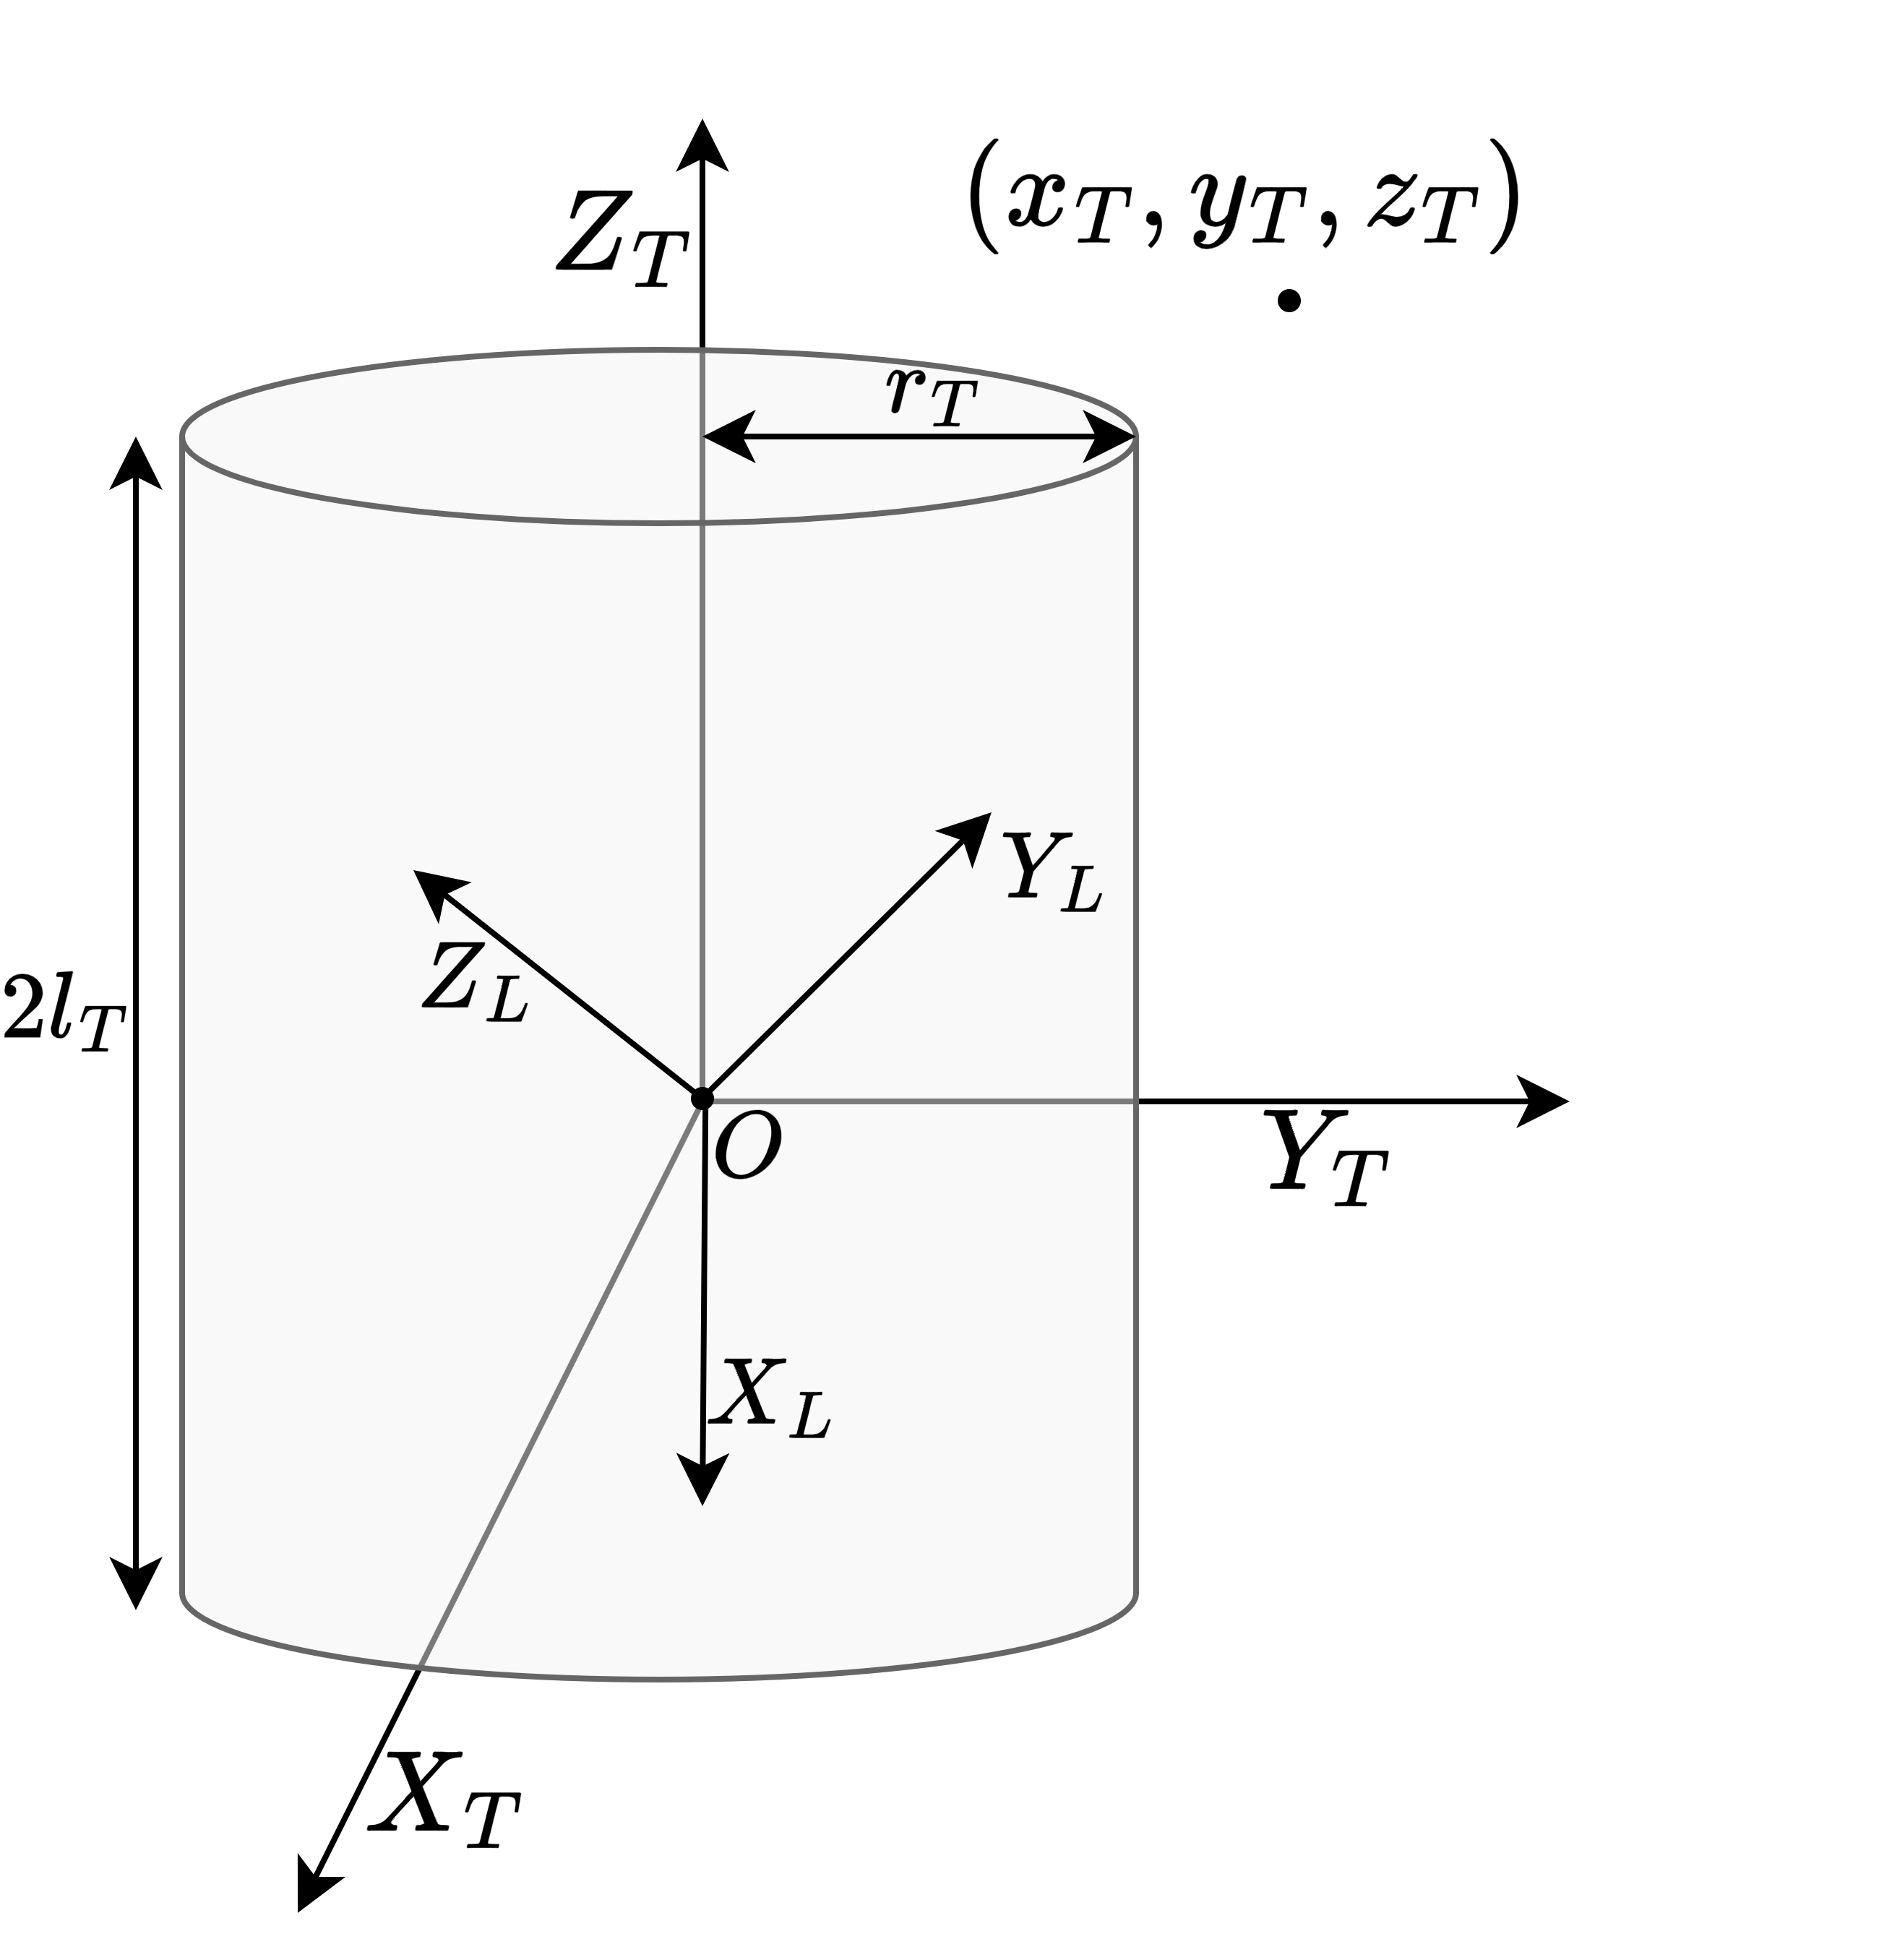
\includegraphics[width=0.9\linewidth]{assets/target-cylinder.png}
    \caption{\textbf{Frames of Reference centered at the Target}: The axes subscripted by $T$ belong to the body frame of the target that rotates with the target and the axes subscripted by $L$ belong to the local-vertical-local-horizontal (LVLH) frame that is defined in Section \ref{sec:relevant-knowledge}}
    \label{fig:target-cylinder}
\end{figure}
The docking operation involves a tighter time-varying state constraint to prevent collisions between the chaser and the target while permitting docking to the boundary of the target.
The same rotational characteristics of the target described in Section \ref{sec:time-varying-final-state-constraint} introduce time-varying collision constraints for the chaser that can be represented as $\boldsymbol{r}(\theta)\in{\mathcal{C}}_D$.
This is motivated by the concept of exclusion from target space as proposed in \cite{park2017nonlinear}.\\
For instance, if the target is cylindrical with radius $r_T$ and length $2l_T$ centered at the origin as demonstrated in Figure \ref{fig:target-cylinder} and rotates such that its rotation matrix at time $t$ is given as $R(t)$, the permissible state set ${\mathcal{C}}_D$ for the chaser can be written as the following union:
\begin{subequations}\label{third:main}
\begin{align}
    {\mathcal{C}}_D&={\mathcal{C}}_{D1}\cup{\mathcal{C}}_{D2}\label{eqn:or-function}\tag{\ref{third:main}}\\
    {\mathcal{C}}_{D1}&=\{\boldsymbol{r}(\theta):f_{D1}=x_{\mathcal{R}}(\theta)^2 + y_{\mathcal{R}}(\theta)^2 - r_T^2\geq0\}\\
    {\mathcal{C}}_{D2}&=\{\boldsymbol{r}(\theta):f_{D2}=||z_{\mathcal{R}}(\theta)|| - l_T\geq0\}
\end{align}
\end{subequations}
where the de-rotated state vector $r_{\mathcal{R}}(\theta)$ (i.e., the position of the chaser as viewed in a target-centered frame of reference that rotates with the target) is defined as:
\begin{align}
    \boldsymbol{r}_{\mathcal{R}}(\theta)&=\begin{bmatrix}
        x_{\mathcal{R}}(\theta)&y_{\mathcal{R}}(\theta)&z_{\mathcal{R}}(\theta)&\dot{x}_{\mathcal{R}}(\theta)&\dot{y}_{\mathcal{R}}(\theta)&\dot{z}_{\mathcal{R}}(\theta)
    \end{bmatrix}^T\notag\\
    &=\left(R^{-1}(\theta)\otimes I_2\right)\boldsymbol{r}(\theta)
\end{align}
Here, $A\otimes B$ represents the Kronecker product of the two matrices $A$ and $B$.
Also, we recall that ${\mathcal{R}}^{-1}={\mathcal{R}}^T$.
The above union can be implemented on a numerical solver using the following logic:
\begin{align}
    {\mathcal{C}}_D=\{\boldsymbol{r}(\theta)\ |\ \text{sgn}(f_{D1})+\text{sgn}(f_{D2})\geq0\}
\end{align}
% The above union can be implemented on a numerical solver as:
% \begin{align}
%     {\mathcal{C}}_D=\{\boldsymbol{r}(\theta)|\max\{{\mathcal{C}}_{D1}, {\mathcal{C}}_{D2}\}\geq0\}.
% \end{align}
% Alternatively, when the $\max$ function is not available, this can be implemented using the following logic:
% \begin{align}
%     {\mathcal{C}}_D=\{\boldsymbol{r}&(\theta)|\notag\\
%     &f_{D1}f_{D2}\left(\left(f_{D1}+f_{D2}\right)-\left(|f_{D1}|+|f_{D2}|\right)\right)\geq0\}
% \end{align}
% or using the following logic:
% \begin{align}
%     {\mathcal{C}}_D=\{\boldsymbol{r}(\theta)|\text{sgn}(f_{D1})+\text{sgn}(f_{D2})\geq0\}
% \end{align}
% such that the logic presented in Table \ref{tab:or-logic} holds.
% \begin{table*}[t]
%     \centering
%     \begin{tabular}{||c|c||c|c||c||}
%     \hline
%         ${\mathcal{C}}_1$ & ${\mathcal{C}}_2$ & ${\mathcal{C}}_1{\mathcal{C}}_2$ & $({\mathcal{C}}_1+{\mathcal{C}}_2)-(|{\mathcal{C}}_1|+|{\mathcal{C}}_2|)$ & ${\mathcal{C}}={\mathcal{C}}_1{\mathcal{C}}_2\left(\left({\mathcal{C}}_1+{\mathcal{C}}_2\right)-\left(|{\mathcal{C}}_1|+|{\mathcal{C}}_2|\right)\right)$ \\
%     \hline
%         + & + & + & 0 & 0 \\
%         + & - & - & - & + \\
%         - & + & - & - & + \\
%         - & - & + & - & - \\
%     \hline
%     \end{tabular}
%     \caption{Implementation of OR Logic in the Optimization Problem}
%     \label{tab:or-logic}
% \end{table*}
\section{Incorporation of Dynamic Tubes for Constraint Satisfaction}
\label{sec:dynamic-tube}
\begin{figure*}[htb]
    \centering
    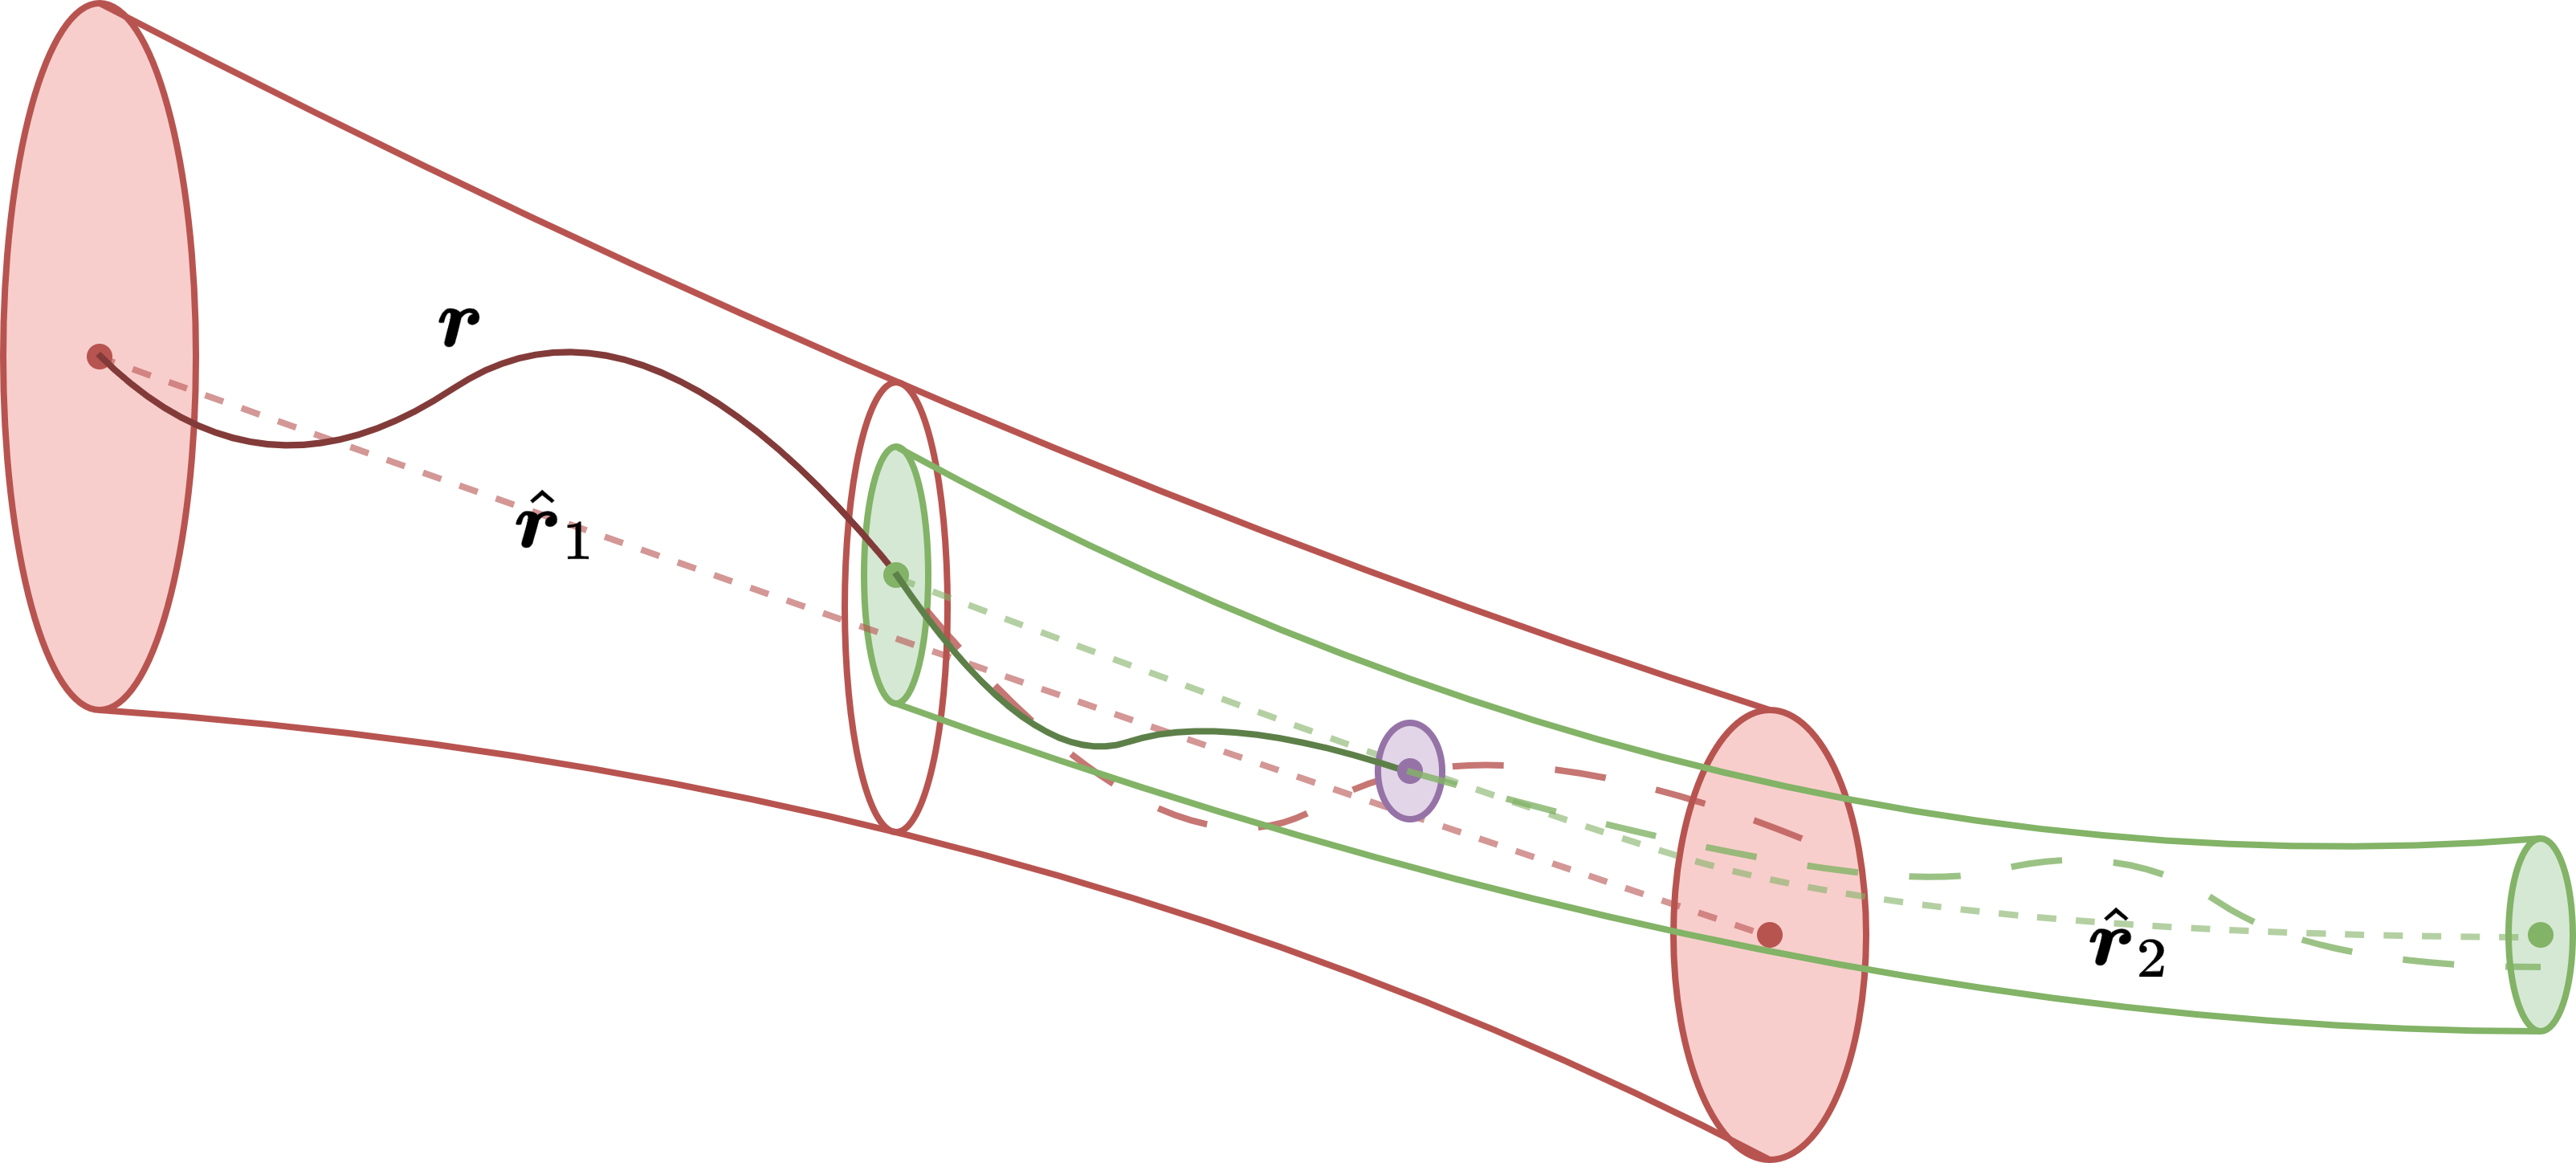
\includegraphics[width = 0.9\textwidth]{assets/adtmpc.png}
    \caption{\textbf{Adaptive Tube Model Predictive Control}: The tubes represent the permissible region for the actual trajectory of the chaser. The dotted lines represent the nominal states and the dashed lines represent the actual states. Due to the receding horizon nature of the problem, the spacecraft plans a new trajectory before the final state is reached.}
    \label{fig:adtmpc}
\end{figure*}
Following the determination of the docking point of the chaser, the chaser plans a trajectory from the current position to the calculated goal position on the target.
By the completion of rendezvous, the chaser has a significantly accurate estimate for uncertain parameters such as eccentricity and drag coefficients and it is capable of planning a trajectory from a start position to a docking point on the target.
However, the high degree of proximity and physical contact required for docking increases the likelihood of a chaser-target collision.
This is theoretically avoided using the time-varying docking constraint explained in Section \ref{sec:time-varying-collision-constraints}.
However, the inaccuracy in estimated parameters may lead to a violation of this constraint.
In order to avoid such constraint violations, we use dynamic robust control-invariant (RCI) tubes as proposed in \cite{brett2019dynamic} to constrain the possible error in the chaser state, hence using adaptive dynamic tube MPC (ADTMPC) for chaser trajectory planning.
As a result, the nominal trajectory planning problem for docking can be formulated as the following optimization problem:
\begin{align}
    \min_{\hat{\boldsymbol{r}}, \hat{\boldsymbol{u}}, \hat{\boldsymbol{v}}}\ &J(\hat{\boldsymbol{r}}(\theta),\hat{\boldsymbol{u}}(\theta))=\int_{\theta_0}^{\theta_f}\left(\hat{\boldsymbol{u}}^T(\theta)R\hat{\boldsymbol{u}}(\theta)\right)d\theta
\end{align}
\begin{subequations}
\begin{align}
    \textrm{s.t. } & \hat{\boldsymbol{r}}'(\theta)=A(\theta)\hat{\boldsymbol{r}}(\theta)+B(\theta)\hat{\boldsymbol{u}}(\theta)+\hat{\boldsymbol{d}}(\theta), \ \ \hat{\boldsymbol{u}}\in\hat{\mathbb{U}},\\
    & \hat{\boldsymbol{r}}(\theta_0)=\boldsymbol{r}(\theta_0)=\boldsymbol{r}_0, \quad\zeta(\hat{\boldsymbol{r}}(\theta_f))=0,\quad{\mathcal{C}}>0,\\
    & \hat{\boldsymbol{\alpha}}'(\theta)=\hat{\boldsymbol{v}}(\theta), \ \ \hat{\boldsymbol{\alpha}}(\theta_0)=\boldsymbol{\alpha}_0, \ \ \hat{\boldsymbol{\alpha}}(\theta)\in{\mathbb{A}}, \ \ \hat{\boldsymbol{v}}(\theta)\in{\mathbb{V}},\\
    & \boldsymbol{\phi}'(\theta)=-[\hat{\boldsymbol{\alpha}}(\theta)][\boldsymbol{\phi}(\theta)]+\boldsymbol{\Delta}(\hat{\boldsymbol{r}}(\theta))+\boldsymbol{D}+\boldsymbol{\eta},\ \ \boldsymbol{\phi}(\theta_0)=\boldsymbol{\phi}_0,\\
    & \boldsymbol{\Omega}'(\theta)=A_\lambda\boldsymbol{\Omega}(\theta)+B_\lambda\boldsymbol{\phi}(\theta),\quad\boldsymbol{\Omega}(\theta_0)=|\Tilde{\boldsymbol{r}}_0|
    \label{eqn:docking-problem}
\end{align}
\end{subequations}
where $A_\lambda=\text{diag}(\boldsymbol{\lambda})=\text{diag}(\{\lambda_i,i=1,2,3\})$ and $B_\lambda=I_{3}$ are predefined, and $[\boldsymbol{v}]=\text{diag}(\boldsymbol{v})$ for a vector $\boldsymbol{v}$.
Here, $\phi(\theta)$ represents the boundary layer of the tube and $\Omega(\theta)$ represents the tube geometry.
\subsection{Ancillary Controller and the Actual Control Input}
In light of the proposed uncertainties and the dynamic tube mechanism to deal with them, we implement control input modification as proposed originally in the DTMPC algorithm \cite{brett2019dynamic} since it provides recursive feasibility to the MPC problem.
The actual control input $\boldsymbol{u}$ can be written as the sum of the nominal input $\hat{\boldsymbol{u}}$ and an ancillary controller $\Tilde{\boldsymbol{u}}$ based on boundary-layer sliding control (BLSC):
\begin{alignat}{2}
    \boldsymbol{u}&=\hat{\boldsymbol{u}}+\Tilde{\boldsymbol{u}}\\
    \Tilde{\boldsymbol{u}}&=B(\boldsymbol{r})^{-1}\left(A^V\Tilde{\boldsymbol{r}}-A_\lambda\Tilde{\boldsymbol{r}}^V-[K(\boldsymbol{r})]\left[\text{sat}\left(\frac{\boldsymbol{s}}{\boldsymbol{\phi}}\right)\right]\right)
\end{alignat}
where the sliding variable $\boldsymbol{s}$ is defined as:
\begin{alignat}{2}
    \boldsymbol{s}=\Tilde{r}^V+A_\lambda\Tilde{r}^P,
\end{alignat}    
and $K(\boldsymbol{r})$ can be calculated as:
\begin{alignat}{2}
    \boldsymbol{\phi}'&=-[\boldsymbol{\alpha}][\boldsymbol{\phi}]+\boldsymbol{\Delta}(\boldsymbol{r}(\theta))+\boldsymbol{D}+\boldsymbol{\eta}\\
    K(\boldsymbol{r})&=\boldsymbol{\Delta}(\boldsymbol{r}(\theta))+\boldsymbol{D}+\boldsymbol{\eta}-\phi'\\
    &=(\boldsymbol{\Delta}(\boldsymbol{r}(\theta))-\boldsymbol{\Delta}(\hat{\boldsymbol{r}}(\theta)))+[\boldsymbol{\alpha}][\boldsymbol{\phi}]\\
    &=\boldsymbol{\Delta}(\Tilde{\boldsymbol{r}}(\theta))+[\boldsymbol{\alpha}][\boldsymbol{\phi}].\label{eqn:K(r)}
\end{alignat}
Here, $\boldsymbol{\Delta}(\boldsymbol{r}(\theta))$ is the maximum bound on the dynamics $\boldsymbol{f}=\hat{\boldsymbol{f}}+\Tilde{\boldsymbol{f}}$ where $\hat{\boldsymbol{f}}$ is the nominal dynamics and $\Tilde{\boldsymbol{f}}$ is the bounded model error such that $|\Tilde{\boldsymbol{f}}|\leq\boldsymbol{\Delta}(\boldsymbol{r}(\theta))$.
Also, $\boldsymbol{D}$ is the maximum bound on the disturbance $\boldsymbol{d}(\theta)$ in the dynamics such that $\boldsymbol{d}(\theta)\leq\boldsymbol{D}$, and $\boldsymbol{\eta}$ is a predefined quantity.
\subsection{Shrinking of State and Input Bounds}
\label{sec:bound-shrinking}
State and input constraints need to be modified due to the non-zero tracking error $\Tilde{\boldsymbol{r}}(\theta)$. The state and input bounds defined in Section \ref{sec:state-input-bounds} must be modified to account for the non-zero tracking error and control input error. We incorporate the tightening equations proposed in \cite{brett2019dynamic} as follows:
\begin{align}
    ||P_{\hat{\boldsymbol{r}}}\boldsymbol{r}(\theta)+q_{\hat{\boldsymbol{r}}}||&\leq C_{\hat{\boldsymbol{r}}}-||P_{\hat{\boldsymbol{r}}}\Tilde{\boldsymbol{r}}(\theta)||\\
    ||P_{\hat{\boldsymbol{u}}}\overline{B}^{-1}\hat{\boldsymbol{u}}(\theta)+q_{\hat{\boldsymbol{u}}}||&\leq C_{\hat{\boldsymbol{u}}}-||P_{\hat{\boldsymbol{u}}}\overline{B}^{-1}\Tilde{\boldsymbol{u}}_{fb}||
\end{align}
In our problem, we may write this (for $i=1,2,3$) as:
% \begin{align}
%     ||\boldsymbol{r}^P(t)||_\infty&<    \infty\quad\text{(no bound)}\\
%     ||\boldsymbol{r}^V(t)||_\infty&\leq C_{\boldsymbol{r}^V}-||\boldsymbol{r}^V(t)||_\infty\\
%     ||\boldsymbol{u}  (t)||_\infty&\leq C_{\boldsymbol{u}}
% \end{align}
\begin{align}
    |r_i^P(\theta)|&<    \infty\quad\text{(no bound)},\\
    |r_i^V(\theta)|&\leq C_{r^V}-|\Tilde{r}^V|,\\
    |u_i  (\theta)|&\leq C_{u}-|\Tilde{u}_{fb,i}|,
\end{align}
such that
\begin{subequations}\label{fourth:main}
\begin{alignat}{2}
    \Tilde{\boldsymbol{u}}_{fb}&=\left|\overline{F}+A_{\lambda}\Tilde{\boldsymbol{r}}\right.&&\left.+\overline{K}\right|\tag{\ref{fourth:main}}\\
    \overline{\boldsymbol{F}}&=A^V\overline{\boldsymbol{r}},&&\underline{\boldsymbol{F}}=A^V\underline{\boldsymbol{r}}\\
    \overline{\boldsymbol{K}}&=K\left(\overline{\boldsymbol{r}}\right),&&\underline{\boldsymbol{K}}=K\left(\underline{\boldsymbol{r}}\right)\\
    \overline{\boldsymbol{r}}&=\hat{\boldsymbol{r}}+|\Tilde{\boldsymbol{r}}|,&&\underline{\boldsymbol{r}}=\hat{\boldsymbol{r}}-|\Tilde{\boldsymbol{r}}|
\end{alignat}
\end{subequations}
where $K(\cdot)$ is defined in Equation \ref{eqn:K(r)}.
\subsection{Expansion of (Concave) State Constraints}
We realize that, although the inputs are bound in a convex space, the state space is non-convex either due to the radial-limit constraint (Equation \ref{eqn:radial-limit-constraint}) during rendezvous or due to the target-limit constraint (Section \ref{sec:time-varying-collision-constraints}) during docking.
These constraints need to be expanded resembling how the convex bounds are shrunk in Section \ref{sec:bound-shrinking}.
As a result, the radial-limit constraint can now be rewritten as:
\begin{align}
    ||\boldsymbol{r}^P(\theta_f)||>r_{\text{Target}}+||\Tilde{\boldsymbol{r}}^P|| \label{eqn:expanded-radial-limit-constraint}
\end{align}
Now, the target-limit constraint must be expanded such that the dynamic RCI tube can at most touch the target.
However, since distances are invariant to rotations, the expansion of the constraint is not affected by the rotation of the position of the chaser with respect to the target.
As a result, the target-limit constraint in Equation \ref{eqn:or-function} can be rewritten as follows:
\begin{subequations}\label{fifth:main}
\begin{align}
    {\mathcal{C}}_D&={\mathcal{C}}_{D1}\cup{\mathcal{C}}_{D2}\label{eqn:expanded-target-limit-constraint}\tag{\ref{fifth:main}}\\
    {\mathcal{C}}_{D1}&=\{\boldsymbol{r}(\theta):f_{D1}\geq0\}\\
    {\mathcal{C}}_{D2}&=\{\boldsymbol{r}(\theta):f_{D2}\geq0\}
\end{align}
\end{subequations}
where
\begin{subequations}
\begin{align}
    f_{D1}&=x_{\mathcal{R}}(\theta)^2 + y_{\mathcal{R}}(\theta)^2 - (r_T+||\Tilde{\boldsymbol{r}}^P||)^2\\
    f_{D2}&=||z_{\mathcal{R}}(\theta)|| - (l_T+||\Tilde{\boldsymbol{r}}^P||)
\end{align}
\end{subequations}
We realize that this can be slightly conservative on the edges of the target.
This can be rectified by adding a third constraint while ignoring the existing two constraints at the edge to provide a rounded cylinder constraint.
We do not address the equations for the same here but encourage the reader to do the same.
Moreover, it can be made less conservative by constraining each dimension separately, giving:
\begin{subequations}
\begin{align}
    f_{D1}&=x_{\mathcal{R}}(\theta)^2 + y_{\mathcal{R}}(\theta)^2 - (r_T+||\begin{bmatrix}
        \Tilde{x}_{\mathcal{R}}&\Tilde{y}_{\mathcal{R}}
    \end{bmatrix}||)^2\\
    f_{D2}&=||z_{\mathcal{R}}(\theta)|| - (l_T+||\Tilde{z}_{\mathcal{R}}||)
\end{align}
\end{subequations}
where, for $r_i\in[x,y,z]$,
\begin{align}
    \Tilde{r}_{i, {\mathcal{R}}}=r_{i, {\mathcal{R}}}(\theta)-\hat{r}_{i, {\mathcal{R}}}(\theta)
\end{align}
\section{Extension to Multi-Chaser Systems}
\label{sec:multi-agent}
Although several uncontrollable objects in orbit are relatively small, some of the most concerning ones (with respect to the risk they pose to vital controllable systems) are large rocket bodies \cite{mcknight2021identifying}.
A single chaser that may be as large as a conventional satellite may not be capable of providing sufficient thrust or leverage to detumble such an object.
As a result, we propose the use of multiple chasers to simultaneously act on the target for tumble minimization and deorbiting.
In the process of rendezvous and docking, such a multi-agent system will require additional constraints to prevent collisions between themselves and the allocation of similar docking positions on the target.\\
% Furthermore, during rendezvous, it may be optimal for the chasers to view the target from different angles to maximize information regarding the shape and inertial parameters of the target to decide docking points for the chasers.
% We address the addition of inter-chaser constraints and basic observation techniques in this section.
% \subsection{Modifications to the Rendezvous and Docking Problem}
The separate implementation of the rendezvous and docking problem proposed in Sections \ref{sec:chaser_ampc} and \ref{sec:constraints} for each chaser in a multi-agent context introduces the risk of collisions between chasers along with the already-addressed issue of collisions between the chaser and the target as well as the possibility of multiple chasers picking the same docking point.
For the multi-agent problem, the split-up problem of distributed optimization followed by distributed task/goal allocation followed by individual trajectory planning may be different in solution and hence in optimality from the combined problem of distributed optimal control.
The former fails to consider the position of non-ego agents for each individual trajectory planning problem, hence posing the risk of collision.
As a result, we suggest the use of the combined problem of distributed optimal control where the same problem is solved by each chaser based on the initial state of all chasers and a common final state manifold.
Moreover, the problem requires focusing on minimizing the total cost of the operation instead of the individual costs of each chaser.
On the other hand, this brings up the possibility of resource depletion for individual chasers due to which the total control input over time needs to be constrained.
As a result, the multi-agent problem for rendezvous can be written as follows:
\begin{align}
    \min_{\boldsymbol{r}, \boldsymbol{u}}\quad &J(\boldsymbol{r}(\theta),\boldsymbol{u}(\theta))\\
    & =\sum_{i=1}^{N_C}\Big(h(\boldsymbol{r}_i(\theta_f))\notag\\
    & \quad\ +\int_{\theta_0}^{\theta_f}\left(\boldsymbol{r}_i^T(\theta)Q_i\boldsymbol{r}_i(\theta)+\boldsymbol{u}_i^T(\theta)R_i\boldsymbol{u}_i(\theta)\right)d\theta\Big)\notag
\end{align}
\begin{subequations}
\begin{align}
    \textrm{s.t. } & \boldsymbol{r}_i'(\theta)=A(\theta)\boldsymbol{r}_i(\theta)+B(\theta)\boldsymbol{u}_i(\theta)+\boldsymbol{d}(\theta),\\
    & \boldsymbol{r}_i(\theta_0)={\boldsymbol{r}}_{i,0},\quad\quad\boldsymbol{u}_i\in{\mathbb{U}}_i,\\
    & \boldsymbol{r}(\theta)\in{\mathcal{C}}_{i,T}\qquad\quad\ \boldsymbol{r}(\theta)\in{\mathcal{C}}_{i,j}\label{eqn:multi-agent-rendezvous}
\end{align}
\end{subequations}
where $i,j\in[1,2,\ldots,N_C]$ and $j>i$.
Here, while the chaser-target collision constraints, ${\mathcal{C}}_{i,T}$, can be expanded as explained in Section \ref{sec:time-varying-collision-constraints}, the inter-chaser collision constraints can be written as follows:
\begin{align}
    {\mathcal{C}}_{i,j}&=\{\boldsymbol{r}_i(\theta):||\boldsymbol{r}^P_{i}-\boldsymbol{r}^P_{j}||-\epsilon_{i,j}\}
\end{align}
where $\epsilon_{i,j}$ is predetermined based on the geometry of chasers $i$ and $j$. A similar multi-agent problem can be written for the docking problem by replacing the chaser-target collision constraint accordingly.

% \subsection{Observation Shape and Size} \label{ssec:observation-shape}
% Although we propose the optimal positioning of chasers for the observation of and approach toward the target, we employ existing techniques such as that proposed in \cite{setterfield2018inertial} for the estimation of inertial parameters of the target.

% \subsection{Individual Goal State Determination} \label{ssec:goal-state-determination}
% The goal state (position and velocity) of each chaser is determined to lie on an observation sphere of optimal radius as discussed in Section \ref{ssec:observation-shape}

\iffalse{
\subsection{Observation Shape and Size}
\label{sec:obs_sphere}
Before the final step of docking with the target, in order to obtain information regarding the mass, moment of inertia, possible locations for docking, and other quantities pertaining to the target vital for the operation, the rendezvous problem may involve intermediate goal points on progressively shrinking concentric surfaces as depicted in Fig. \ref{fig:obs_spheres}.
\begin{figure}[hbt!]
    \centering
    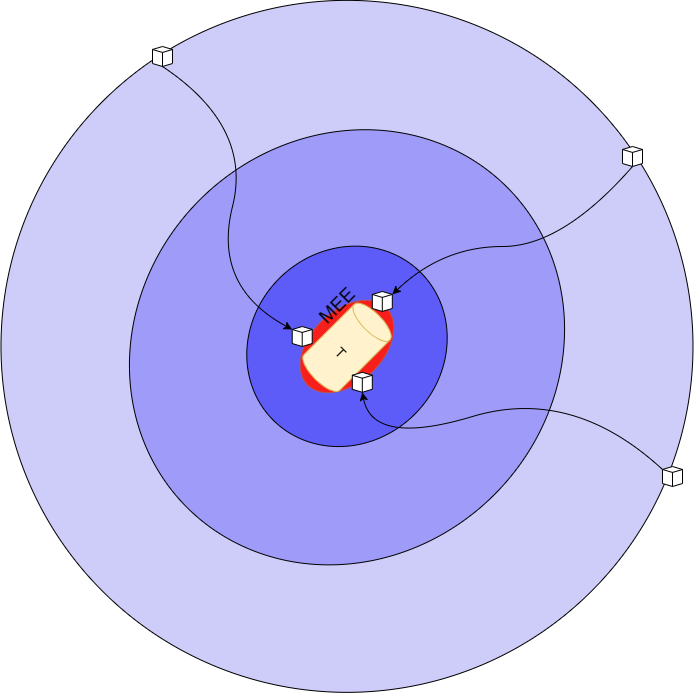
\includegraphics[width=.75\linewidth]{assets/obs-spheres.png}
    \caption{\textbf{Observation and Approach of Chasers onto the Target.} The chasers collect and share information regarding the target as they approach it at each observation surface.}
    \label{fig:obs_spheres}
\end{figure}
In order to calculate optimal positions for chasers to observe the target, we propose a nonlinear optimization problem that aims to maximize the observability of the target.
We draw motivation from multi-satellite implementations for remote sensing and similar works \cite{chen2020a,gu2023large} to define the observability of the target as a heuristic that is proportional to the fraction of area of the target that is observed.
It is easy to realize that the fraction of observed area is proportional to the spread between the chasers at any fixed distance from the target.
% Moreover, given a fixed number of concentric observation surfaces, it may be preferable to distribute the surfaces as far from each other as possible to support easier transit from one surface to the next.
As a result, we define observability as follows while encouraging the reader to explore the possibility of more optimal measurements of observation:
\begin{align}
    {\mathcal{O}}&=Q_{\text{local}}{\mathcal{O}}_{\text{local}}+Q_{\text{cross}}{\mathcal{O}}_{\text{cross}}\\
    {\mathcal{O}}_{\text{local}}&=\sum_{l=1}^{N_L}\sum_{i=1}^{N_C}\sum_{j=i}^{N_C}\left(||\boldsymbol{r}_{i,l}^P-\boldsymbol{r}_{j,l}^P||\right)\\
    {\mathcal{O}}_{\text{cross}}&=\sum_{l=2}^{N_L}\sum_{i=1}^{N_C}\left(-||\boldsymbol{r}_{i,l}^P-\boldsymbol{r}_{i,l-1}^P||\right)
\end{align}
where $\boldsymbol{r}_{i,l}^P$ is the position (in all three axes) of agent $i$ at the $l$th observation surface.
% \begin{equation}
%     \mathcal{O}(\mathcal{S}, \{p_i(t)\forall i\in\mathbb{N}\}(t) \begin{cases} < 1 &\text{for a net loss of information}\\
%                                                                                = 1 &\text{for no net gain or loss of information}\\
%                                                                                > 1 &\text{for a net gain of information}
%                                                                  \end{cases}
% \end{equation}

Now, with the ellipsoid ${\mathcal{E}}_T$ of parameters $a_T, b_T, c_T$ as the final state constraints and a starting ellipsoid ${\mathcal{E}}_0$ of parameters $a_0, b_0, c_0$ such that all the chasers start from points that lie on $\mathcal{E}_0$, we solve the following minimization problem to obtain the optimal observation ellipsoids:
\begin{equation}
\begin{aligned}
    \min_{a_l, b_l, c_l}\quad &J_E=\sum_{l=1}^{N_L-1}{\mathcal{O}}({\mathcal{E}}_l, \{p_{i,l} \forall\ i\in{\mathbb{N}}_C\})\\
    \textrm{s.t. } & a_{l}\leq a_{l-1},\ \ b_{l}\leq b_{l-1},\ \  c_{l}\leq c_{l-1},\ \ \forall\ l\in{\mathbb{N}}_L\\
    & \frac{x_{i,l}^2}{a_l^2}+\frac{y_{i,l}^2}{b_l^2}+\frac{z_{i,l}^2}{c_l^2}=1\ \ \forall\ i\in{\mathbb{N}}_C, l\in{\mathbb{N}}_L
    \label{eqn:mee}
\end{aligned}
\end{equation}
Although we propose the optimal positioning of chasers for the observation of the target and their approach to the target, we employ existing techniques such as those proposed in \cite{setterfield2018inertial} for the estimation of the inertial parameters of the target.
}
% \begin{figure*}
% \centering
% \includegraphics[width=4in]{Placeholder.eps}
% \caption{\bf{Here is an example of a figure that spans both columns.}}
% \label{FlowChart}
% \end{figure*}

% \begin{table}
% \renewcommand{\arraystretch}{1.3}
% \caption{\bf Summary of Due Dates}
% \label{DueDates}
% \centering
% \begin{tabular}{|c|c|}
% \hline
% \bfseries Event & \bfseries Due Date \\
% \hline\hline
% Abstracts Due               & July 1, 2023 \\
% Draft Paper {\bf Deadline} & October 6, 2023 \\
% Revised papers Due          & January 12, 2024\\
% IEEE Copyright Form Due     & January 12, 2024\\
% \hline
% \end{tabular}
% \end{table}
% One figure containing six subfigures one for each positional state (three for rendezvous and three for docking) demonstrates the convergence of the chaser to the final state.
% Move the location of this figure based on placement aesthetics.
\begin{figure*}[htb]
  \begin{subfigure}[b]{0.33\textwidth}
    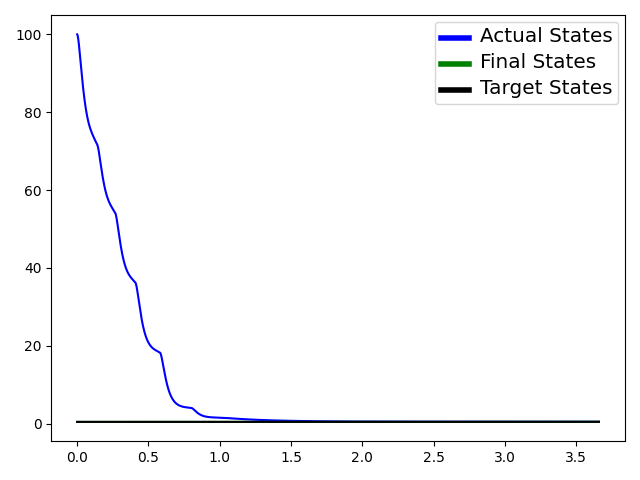
\includegraphics[width=\linewidth]{assets/complete_x_traj.png}
    \caption{Complete Trajectory in the X-axis}
    \label{fig:results_x_rnd}
  \end{subfigure}
  \hfill
  \begin{subfigure}[b]{0.33\textwidth}
    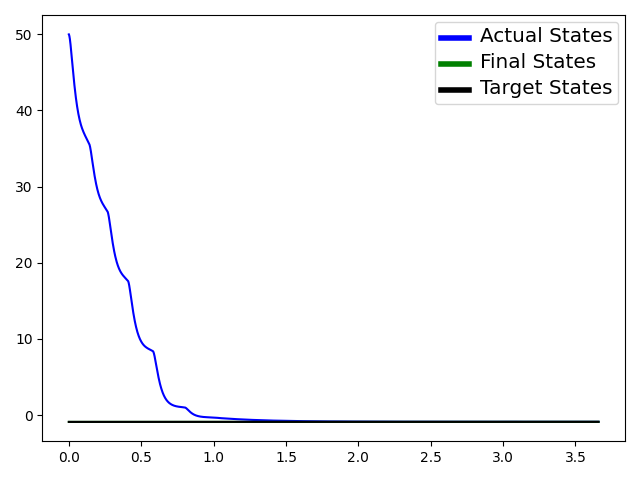
\includegraphics[width=\linewidth]{assets/complete_y_traj.png}
    \caption{Complete Trajectory in the Y-axis}
    \label{fig:results_y_rnd}
  \end{subfigure}
  \hfill
  \begin{subfigure}[b]{0.33\textwidth}
    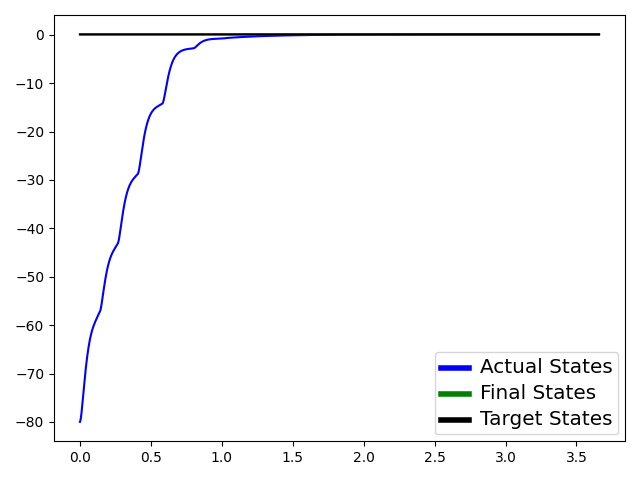
\includegraphics[width=\linewidth]{assets/complete_z_traj.png}
    \caption{Complete Trajectory in the Z-axis}
    \label{fig:results_z_rnd}
  \end{subfigure}
  \begin{subfigure}[b]{0.33\textwidth}
    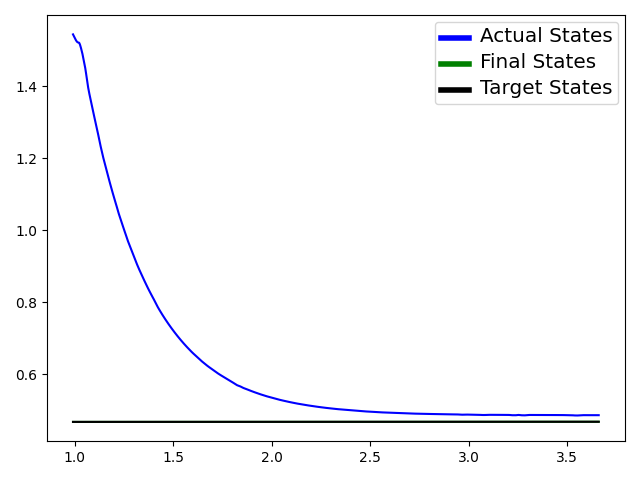
\includegraphics[width=\linewidth]{assets/docking_x_traj.png}
    \caption{Docking Trajectory in the X-axis}
    \label{fig:results_x_dock}
  \end{subfigure}
  \hfill
  \begin{subfigure}[b]{0.33\textwidth}
    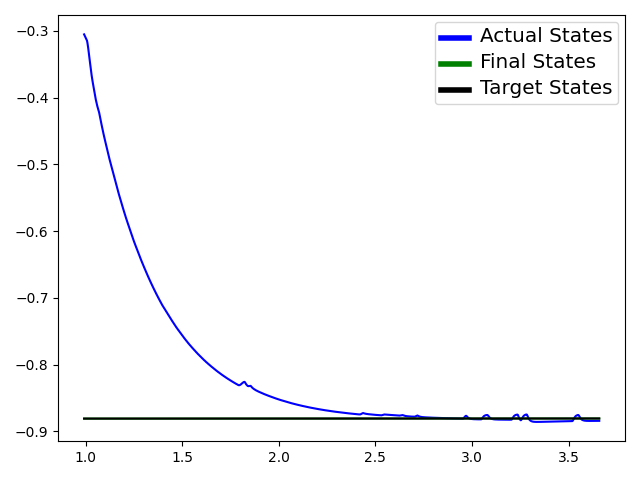
\includegraphics[width=\linewidth]{assets/docking_y_traj.png}
    \caption{Docking Trajectory in the Y-axis}
    \label{fig:results_y_dock}
  \end{subfigure}
  \hfill
  \begin{subfigure}[b]{0.33\textwidth}
    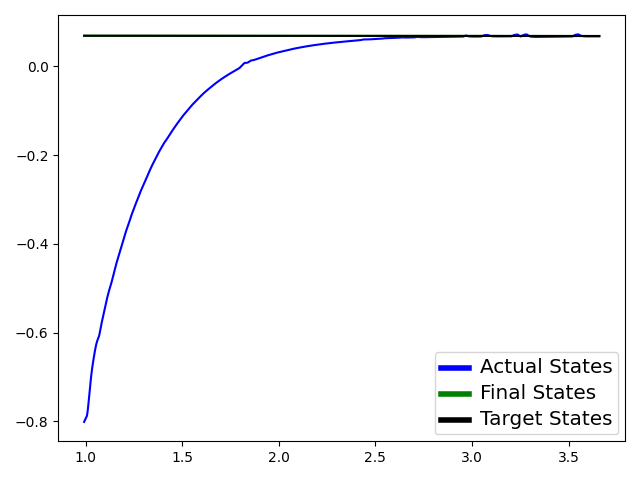
\includegraphics[width=\linewidth]{assets/docking_z_traj.png}
    \caption{Docking Trajectory in the Z-axis}
    \label{fig:results_z_dock}
  \end{subfigure}
  \caption{\textbf{Simulation of Rendezvous and Docking using Adaptive Dynamic Tube Model Predictive Control}: Subfigures \ref{fig:results_x_rnd}, 
 \ref{fig:results_y_rnd}, and \ref{fig:results_z_rnd} demonstrate the positional states of the chaser in the execution of the complete pipeline whereas subfigures \ref{fig:results_x_dock}, \ref{fig:results_y_dock}, and \ref{fig:results_z_dock} focuses on the positional states for the docking operation. Note that rendezvous ends and docking begins when the chaser is at less than 2.0 units away from the docking position.}
 \label{fig:results_pipeline}
\end{figure*}

\section{Target Deflection}
\label{sec:target-deflection}
Once the chaser has docked with the target at some position $\boldsymbol{d}$ with respect to the center of the target, any force $\boldsymbol{f}$ applied by the chaser thrusters translates to a torque $\boldsymbol{\tau}$ applied on the target as:
\begin{align}
    \boldsymbol{\tau} = \boldsymbol{d}\times\boldsymbol{f}
\end{align}
In the multi-agent scenario (with $N_C$ chasers), the net torque acting on the target can be written as:
\begin{align}
    \boldsymbol{\tau} = \sum_{i=1}^{N_C}\boldsymbol{d}_{i}\times\boldsymbol{f}_{i}
\end{align}
As a result, the dynamics of the target can be written using the Newton-Euler equations as follows:
\begin{align}
    \dot{\boldsymbol{\theta}}(t)&=\boldsymbol{\omega}(t)\\
    I\dot{\boldsymbol{\omega}}(t)&=-\boldsymbol{\omega}(t)\times I\boldsymbol{\omega}(t)+\sum_{i=1}^{N_C}\boldsymbol{d}_{i}\times\boldsymbol{f}_{i}
\label{eqn:newton-euler-target-detumbling}
\end{align}
This section focuses on the calculation of the optimal docking position and control input trajectory of the chaser(s) such that the final angular velocity of the target is zero while minimizing a cost function proportional to the net control input.
The interaction of multiple chasers with the target is more complicated than the single-agent case since one agent interacting with the object could change the environment for all other agents.
To simplify this issue, for the multi-agent scenario, we propose the simultaneous attachment of all chasers and the application of thrust so as to stop tumble only after all chasers have been attached to the target.\\
In this section, we retreat to the traditional form of representing, differentiating, and integrating variables with respect to time although the same operations may be performed using true anomaly as the independent variable.
% While the position of a chaser remains stationary after attachment, due to the tumbling nature of the target, the docking onto the target involves a time-varying final-position constraint which is considered in Eqn. \ref{}. For instance, if the target is cylindrical as demonstrated in Fig. \ref{} but revolves about an axis @@@ that does not pass through its center, the final position of each chaser is constrained to the following time-varying cylindrical surface:
% \begin{equation}
% \end{equation}
\subsection{Calculation of Docking Points and Force Application}
In order to calculate the docking points for each chaser $i\in[1,2,\ldots,N_C]$, we minimize the sum of the integral of forces applied by each chaser. This optimal control problem is governed by the Newton-Euler equations described above in Equation \ref{eqn:newton-euler-target-detumbling}. The moment of inertia and the initial angular velocity of the target is obtained from techniques such as polhode analysis as explained in Section \ref{sec:target-estimation}. Since the problem aims to stop the tumble of the target, the final angular velocity of the target is set to zero. Accounting for these constraints, the detumbling problem can be expressed as the following dynamic optimization problem:
\begin{alignat}{2}
    \min_{\boldsymbol{d}_{i},\boldsymbol{f}_{i}}\ &J\left(\boldsymbol{f}_{i}(t),\boldsymbol{d}_{i},\boldsymbol{\theta}_T(t), \boldsymbol{\omega}_T(t)\right)\\
    & =\int_{t_0}^{t_f} C\left(\boldsymbol{f}_{i}(t),\boldsymbol{d}_{i}, \boldsymbol{\theta}_T(t), \boldsymbol{\omega}_T(t)\right) dt\notag\\
    & =\int_{t_0}^{t_f}\sum_{i=1}^N||\boldsymbol{f}_{i}(t)||^2dt\notag
\end{alignat}
\begin{subequations}
\begin{alignat}{2}
    \textrm{s.t. } & \dot{\boldsymbol{\theta}}(t)=\boldsymbol{\omega}(t)\\
    & I\dot{\boldsymbol{\omega}}(t)=-\boldsymbol{\omega}(t)\times I\boldsymbol{\omega}(t)+\sum_{i=1}^{N_C}\boldsymbol{d}_{i}\times\boldsymbol{f}_{i}\\
    & \boldsymbol{\omega}(t_0)=\boldsymbol{\omega}_0,\quad\boldsymbol{\omega}(t_f)=0\\
    & \boldsymbol{f}_{i}\in{\mathbb{F}}_i\\
    & \boldsymbol{d}_C\in{\mathbb{G}}_T \label{eqn:geometrical-constraint}
\end{alignat}
\end{subequations}
Here, ${\mathbb{F}}_i$ represents the input bounds on chaser $i$ and ${\mathbb{G}}_T$ represents the geometrical constraint of the target on the docking point of the chaser. For example, if the target is a cylinder of radius $r_T$ and length $2l_T$ centered at the origin (assuming docking on the curved surface), the geometrical constraint in Equation \ref{eqn:geometrical-constraint} can be expanded as:
\begin{align}
    {\mathbb{G}}_T&={\mathbb{G}}_{T1}\cap{\mathbb{G}}_{T2}\\
    {\mathbb{G}}_{T1}&=\{\boldsymbol{d}_C:\boldsymbol{d}_{C,x}^2+\boldsymbol{d}_{C,y}^2=r_T^2\}\\
    {\mathbb{G}}_{T2}&=\{\boldsymbol{d}_C:|\boldsymbol{d}_{C,z}|<l_T\}
\end{align}
For the problem of calculating docking points, we ignore the rotation of the target. Instead, this rotation is considered in the formulation of the final state constraint for the docking trajectory problem as shown in Section \ref{sec:time-varying-final-state-constraint}.
\subsection{Discretization of Docking Points}
Due to the likelihood that specific points on the target (such as existing docking ports) will support docking better than others, we propose extending the above problem such that the docking position $\boldsymbol{d}_{i}$ lies in a discrete set of positions on the target.
As a result, the continuous geometrical constraint on the position of the chaser given in Equation \ref{eqn:geometrical-constraint} turns into the following discretized constraint:
\begin{align}
    \boldsymbol{d}_{i}&\in\begin{bmatrix}
        \boldsymbol{d}_{T_1}&\boldsymbol{d}_{T_2}&\ldots&\boldsymbol{d}_{T_j}&\ldots&\boldsymbol{d}_{T_M}
    \end{bmatrix}
\end{align}
hence converting the problem to a mixed-integer nonlinear optimal control.
To avoid the complexity involved in solving mixed-integer problems, we define the final position $\boldsymbol{d}_{i}$ for each chaser $i\in[1,2,\ldots,N]$ as follows:
\begin{align}
    o_{i,j}^2-o_{i,j}&=0\ \forall\ j\in[1, 2, \ldots, M]\\
    \sum_{j=1}^Mo_{i,j}&=1\\
    \boldsymbol{d}_{i}&=\sum_{j=1}^Mo_{i,j}\boldsymbol{d}_{T_j},
\end{align}
following which we convert equalities to approximate inequalities for solver convergence:
\begin{align}
    \cdot&=0\iff\lim_{\epsilon\rightarrow0}|\cdot|<\epsilon
\end{align}
\section{Results and Discussion}
\label{sec:results}
This section reports the results of the system proposed in this paper.
The target is considered to be cylindrical in shape considering some of the most statistically-most-concerning (SMC) space debris \cite{mcknight2021identifying} - cylindrical second-stage rocket bodies.
% SL-16s: Zenit second stages that are 4 m in diameter, 12 m in length and 8300 kg in dry mass.
All optimization and optimal control problems are solved using the GEKKO package \cite{beal2018gekko} on Python.
The authors have used both the Advanced Process OPTimizer (APOPT) \cite{hedengren2014nonlinear} and the Interior Point Optimizer (IPOPT) \cite{wachter2006on} solvers based on the speed and computational resource consumption of each problem.

\subsection{The Overall Pipeline}
\label{sec:results_pipeline}
We demonstrate in Figure \ref{fig:results_pipeline} the rendezvous and docking of the chaser with the target using ADTMPC achieving a final positional error of @@@\%.
The adaptation of the unknown parameters 
- the eccentricity of the orbit and the drag coefficient of the target - is noted in Table \ref{tab:parameter-estimation} by including the initial and final estimates and ranges of estimation.
We note that it is possible to obtain more precise simulations of the docking operation by adjusting the cost function matrices and other solver parameters; however, we demonstrate the proof-of-concept of the proposed algorithm.
\begin{table*}[htb]
    \centering
    \begin{tabular}{|c|c|c|c|c|c|}
    \hline
    Parameter                          & Actual Value & Initial Estimate & Final Estimate & Initial Range & Final Range \\
    \hline
    Eccentricity ($\mathsf{e}$)         & $\num{1.25e-1}$ & $\num{0.00e-1}$ & $\num{e-1}$ & $[\num{0.00}, \num{6.00}]\times\num{e-1}$ & $[\num{.00}, \num{.00}]\times\num{e-1}$ \\
    Target Drag Const. ($\alpha$) & $\num{1.30e-7}$ & $\num{0.00e-7}$ & $\num{e-7}$ & $[\num{0.00}, \num{5.00}]\times\num{e-7}$ & $[\num{.00}, \num{.00}]\times\num{e-7}$ \\
    \hline
    \end{tabular}
    \caption{Results: Parameter Estimation via SMID}
    \label{tab:parameter-estimation}
\end{table*}
\begin{figure*}[htb]
  \begin{subfigure}[b]{0.48\textwidth}
    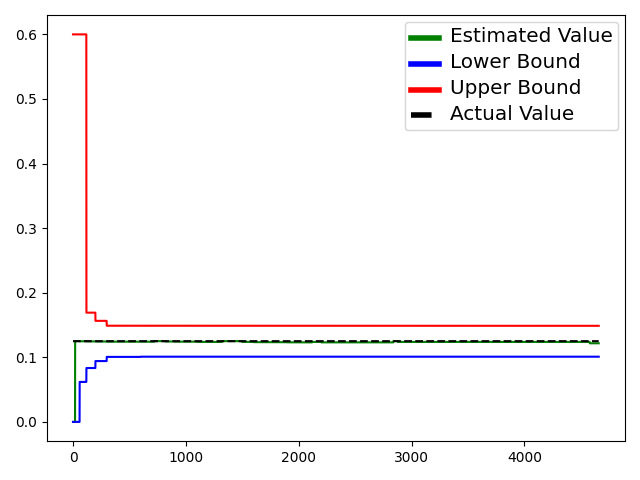
\includegraphics[width=\linewidth]{assets/estim_eccentricity.png}
    \caption{Eccentricity $\mathsf{e}$ of the Orbit}
    \label{fig:results_estim_eccentricity}
  \end{subfigure}
  \hfill
  \begin{subfigure}[b]{0.48\textwidth}
    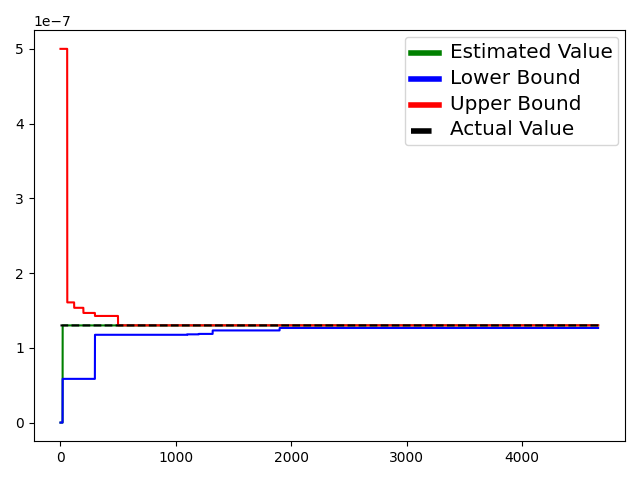
\includegraphics[width=\linewidth]{assets/estim_alpha.png}
    \caption{Estimation of the Drag Constant $\alpha$ of the Target over time}
    \label{fig:results_estim_alpha}
  \end{subfigure}
  \caption{\textbf{Estimation of Unknown Parameters Over Time}}
\end{figure*}

\subsection{Analysis of ADTMPC and other techniques}
\label{sec:results_analysis}
We perform the following analysis to depict the advantages of using ADTMPC over plain MPC.
As is visible from Figure \ref{fig:results_tube}, MPC with and without using adaptive control (and hence the estimation of the unknown parameters) leads to the violation of the chaser-target collision constraints.
% One figure containing four subfigures demonstrates the violation of constraints
\begin{figure*}[b]
  \begin{subfigure}[b]{0.49\textwidth}
    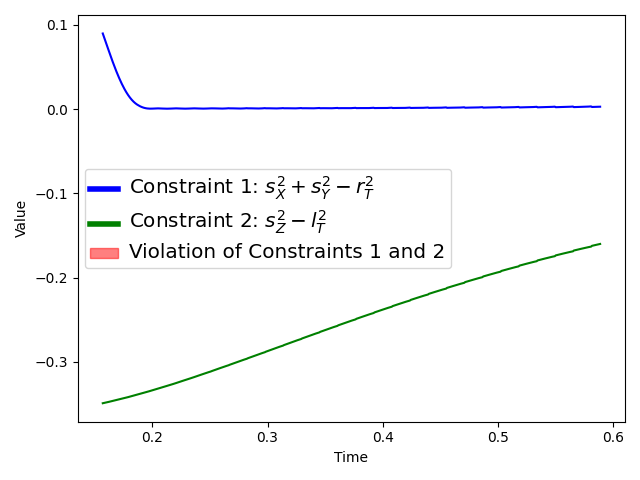
\includegraphics[width=\linewidth]{assets/results_with_tube_dtmpc.png}
    \caption{Dynamic Tube MPC}
    \label{fig:results_with_tube_dtmpc}
  \end{subfigure}
  \hfill
  \begin{subfigure}[b]{0.49\textwidth}
    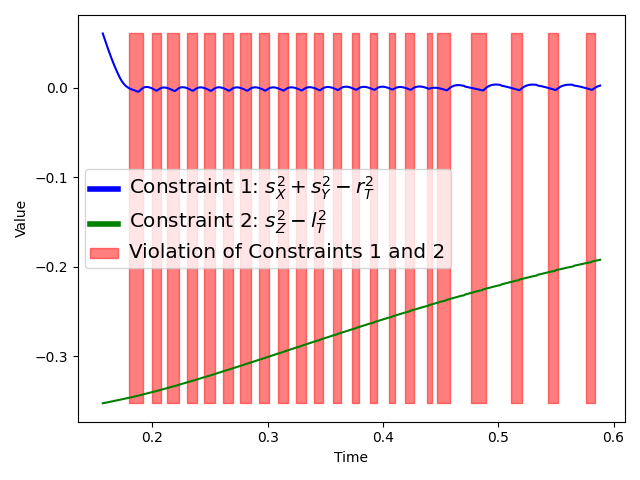
\includegraphics[width=\linewidth]{assets/results_no_tube_mpc.png}
    \caption{MPC (no robust tubes)}
    \label{fig:results_no_tube_mpc}
  \end{subfigure}
  \caption{\textbf{Violation of Collision Constraints without Robust Tubes}: The red regions represent time periods when the collision constraint defined previously as $\boldsymbol{r}(\theta)\in{\mathcal{C}}_D$ is violated.}
  \label{fig:results_tube}
\end{figure*}
Simply using dynamic tubes without adaptation proves to be effective in preventing collisions.
However, due to inaccurate estimates of the unknown parameters and, hence, a large tube, the chaser is unable to converge to the desired docking position on the target.
On the other hand, adaptive dynamic tube MPC shrinks the tube over time, hence allowing the chaser to converge to the final docking position.
Figure \ref{fig:results_adapt} demonstrates how, in very close proximity of the target, previous adaptation of unknown parameters and, hence, a smaller robust tube permits the chaser to move closer to the docking position.
% One figure containing two subfigures one for ADTMPC and the other for DTMPC demonstrates the closeness of the chaser to the target and to the final state.
\begin{figure*}[htb]
  \begin{subfigure}[b]{0.48\textwidth}
    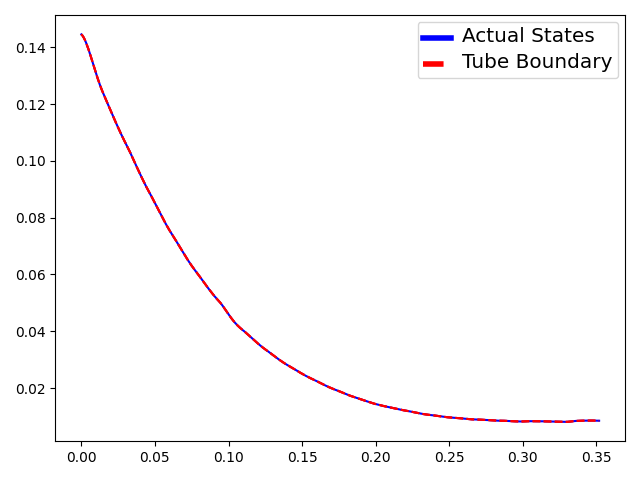
\includegraphics[width=\linewidth]{assets/results_adapt_adtmpc.png}
    \caption{Adaptive Dynamic Tube MPC}
    \label{fig:results_adapt_adtmpc}
  \end{subfigure}
  \hfill
  \begin{subfigure}[b]{0.48\textwidth}
    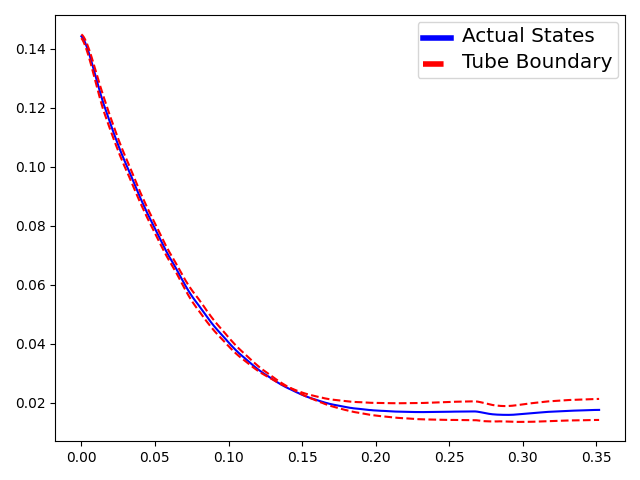
\includegraphics[width=\linewidth]{assets/results_no_adapt_dtmpc.png}
    \caption{Dynamic Tube MPC (no adaptation)}
    \label{fig:results_no_adapt_dtmpc}
  \end{subfigure}
  \caption{\textbf{The Effect of Adaptation}: These plots demonstrate the effect of SMID-based parameter estimation on the size of tubes and, hence, the convergence of the chaser to the final docking point.}
  \label{fig:results_adapt}
\end{figure*}

\subsection{Target Deflection}
\label{sec:results_target_deflect}
Next, we run the optimization problem proposed in Section \ref{sec:target-deflection} such that the chaser attaches to a point within a set of known docking positions and applies a net optimal force to detumble the target.
Figure \ref{fig:results_deflection} demonstrates the results obtained in this regard.
% One figure containing two subfigures one for ADTMPC and the other for DTMPC demonstrates the closeness of the chaser to the target and to the final state.
\begin{figure*}[b]
  \begin{subfigure}[b]{0.22\textwidth}
    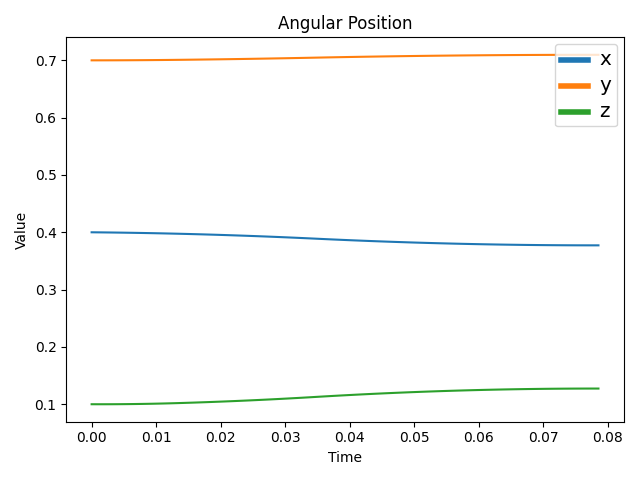
\includegraphics[width=\linewidth]{assets/results_target_angpos.png}
    \caption{Target Angular Position}
    \label{fig:results_target_angpos}
  \end{subfigure}
  \hfill
  \begin{subfigure}[b]{0.22\textwidth}
    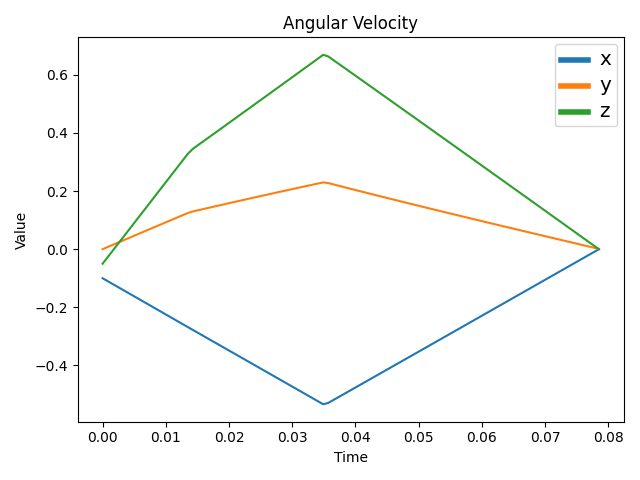
\includegraphics[width=\linewidth]{assets/results_target_angvel.png}
    \caption{Target Angular Velocity}
    \label{fig:results_target_angvel}
  \end{subfigure}
  \hfill
  \begin{subfigure}[b]{0.30\textwidth}
    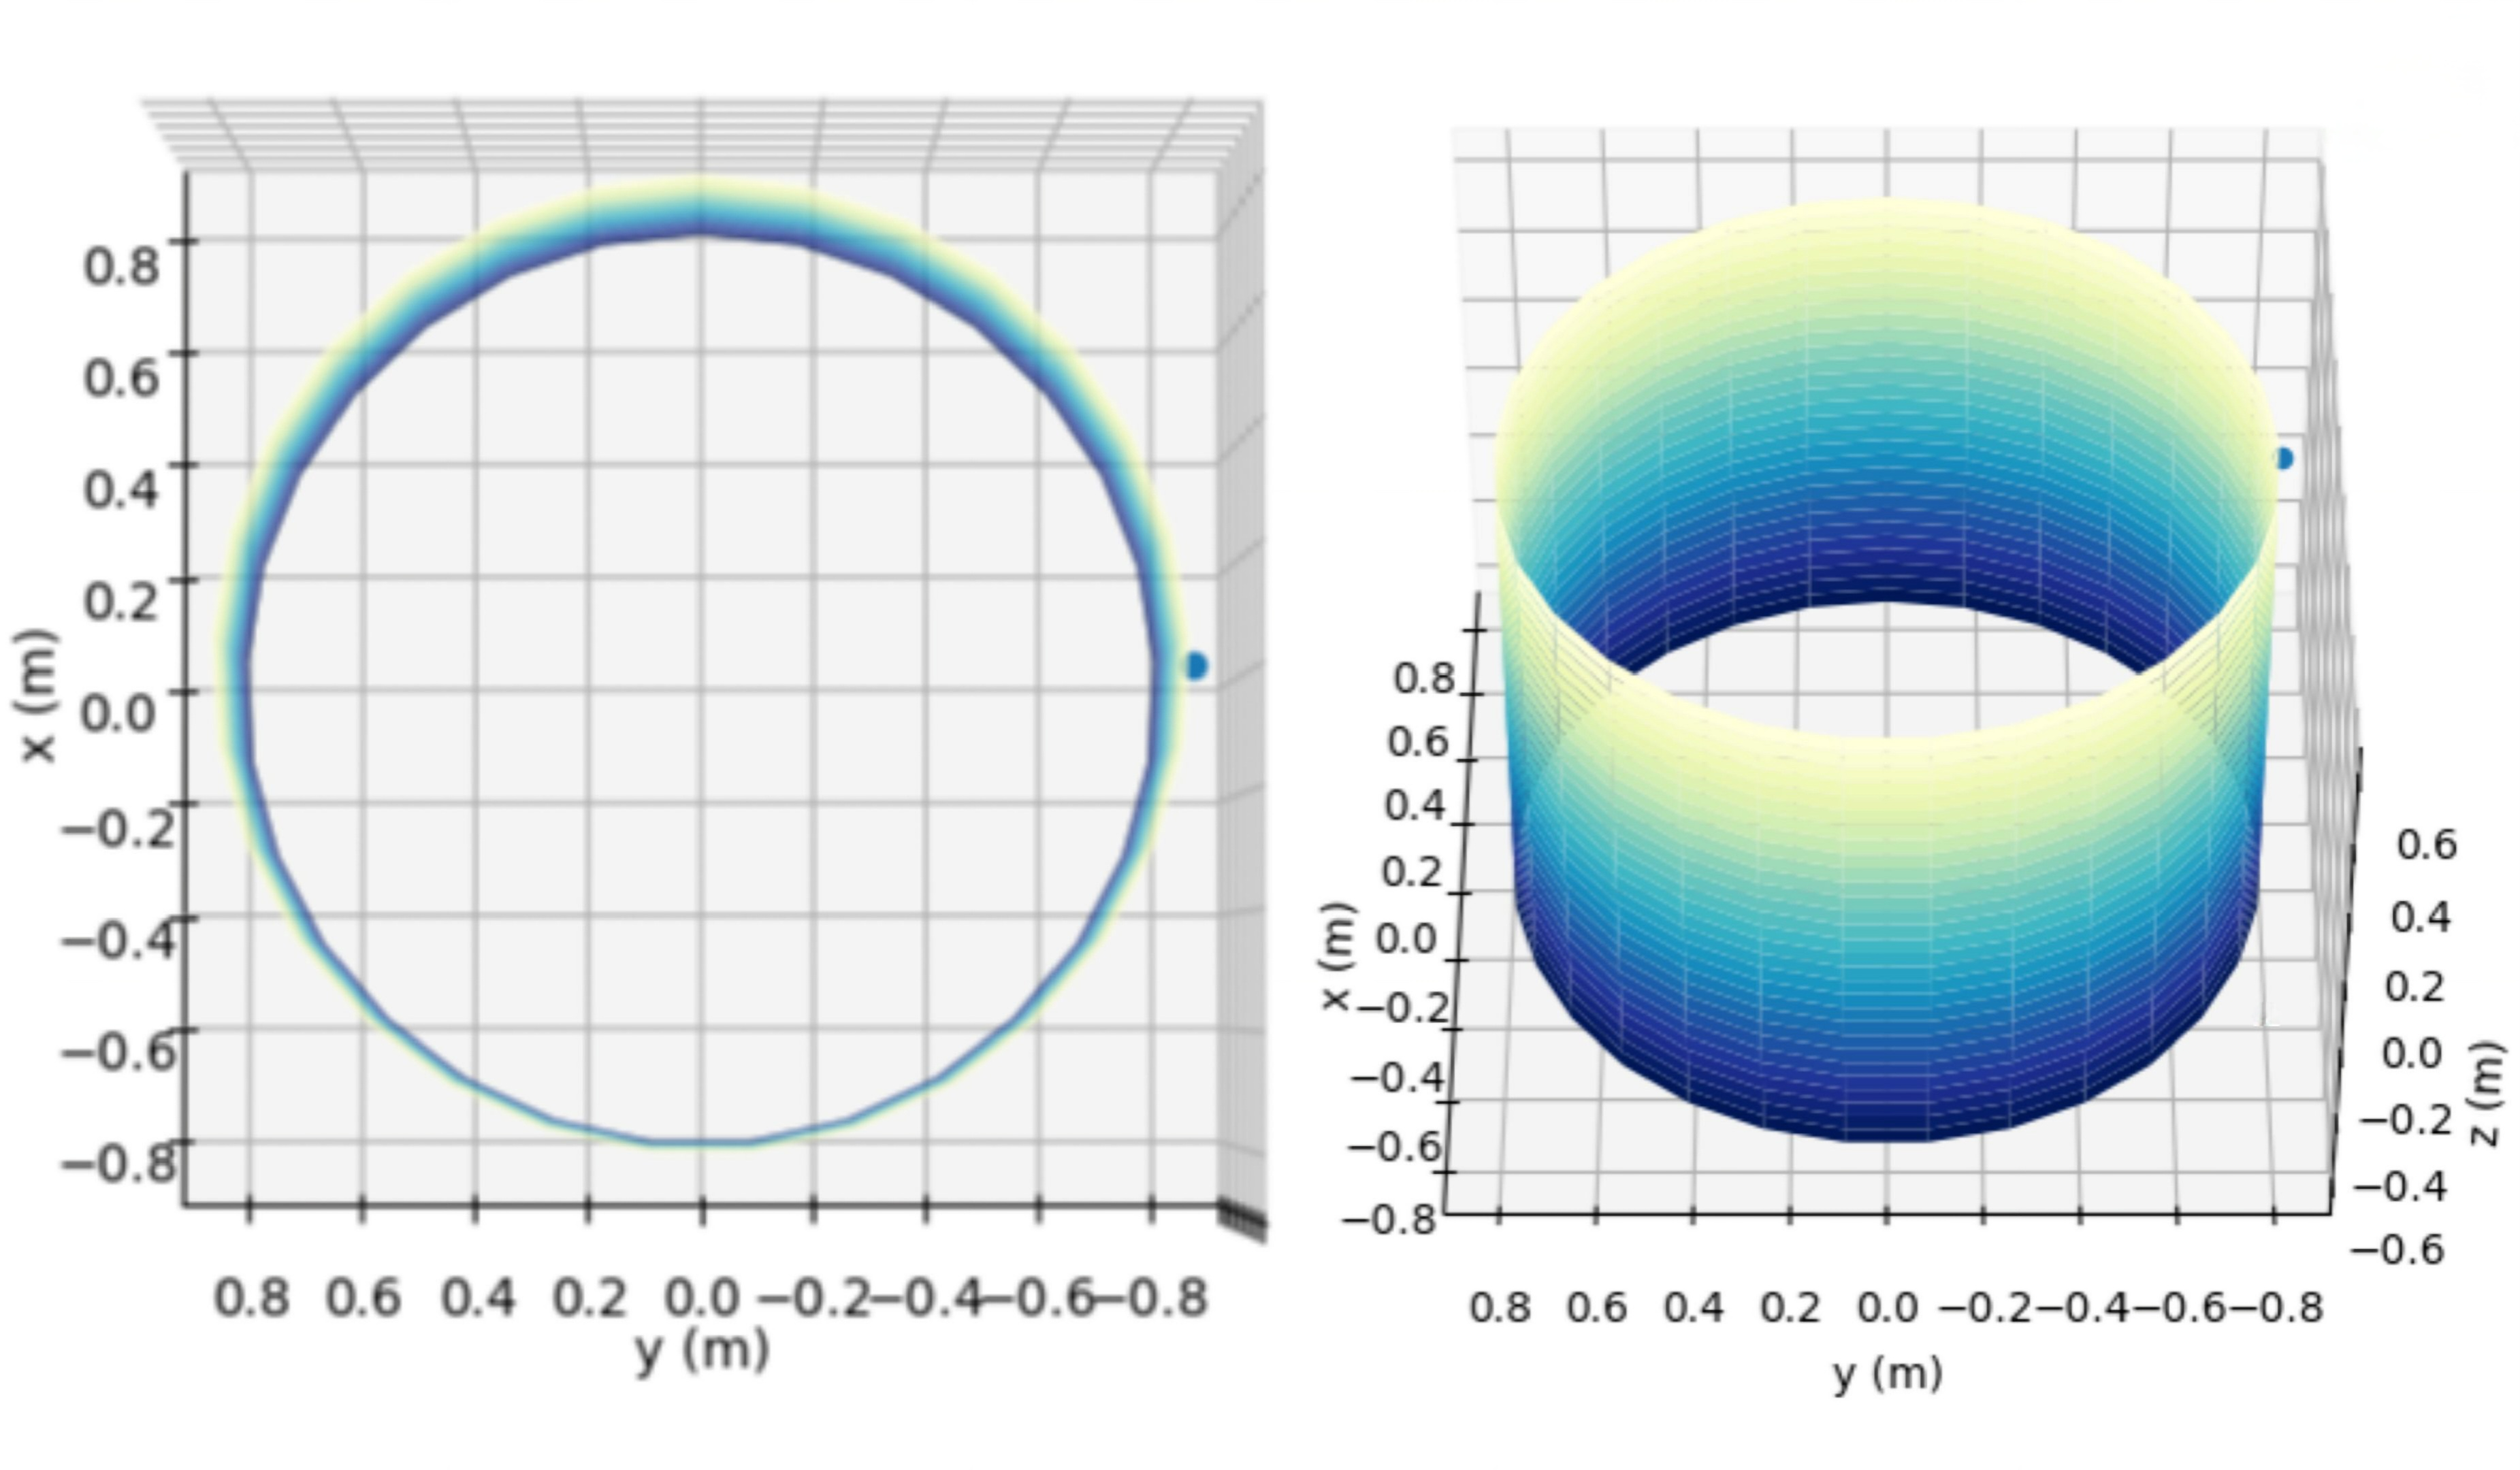
\includegraphics[width=\linewidth]{assets/results_docking_point.jpg}
    \caption{Optimal Chaser Docking Position}
    \label{fig:results_docking_point}
  \end{subfigure}
  \hfill
  \begin{subfigure}[b]{0.22\textwidth}
    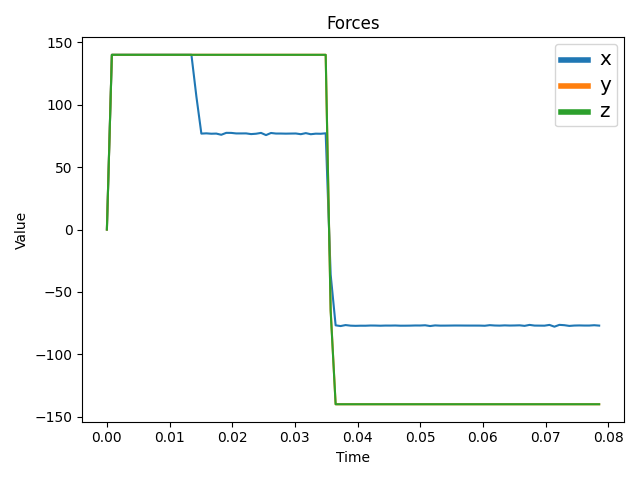
\includegraphics[width=\linewidth]{assets/results_chaser_force.png}
    \caption{Optimal Chaser Force}
    \label{fig:results_chaser_force}
  \end{subfigure}
  \caption{\textbf{Target Deflection}: Subfigures \ref{fig:results_target_angpos} and \ref{fig:results_target_angvel} demonstrate the detumbling of the target such that its angular velocity converges to zero. The blue dot in subfigure \ref{fig:results_docking_point} demonstrates the optimal docking position of the chaser (single-chaser scenario) on the target such that the target is detumbled on the application of force as depicted in subfigure \ref{fig:results_chaser_force}.}
  \label{fig:results_adapt}
\end{figure*}

\iffalse{
\subsection{Observation Spheres}
We do not present results on the implementation of rendezvous and docking using multiple agents.
However, here we demonstrate the calculation of optimal observation spheres given initial and final conditions.
Assuming the target to be a cylinder of radius $r_T=0.6\ u$ and length $l_T=0.8\ u$ (positional units are defined as $u=10\ m$) and the initial ellipsoid to be a sphere of radius $137.5\ u$, the minimum enclosing ellipsoid and hence the final ellipsoid ${\mathcal{E}}_T$ for the optimization problem is defined as:
\begin{align}
    \frac{x^2}{0.980}+\frac{y^2}{0.980}+\frac{z^2}{1.039}=1
\end{align}
We run hyperparameter optimization setting $Q_{\text{local}}=1.0000$ to obtain $Q_{\text{cross}}=0.0960$.
Table \ref{tab:ch5-res-chaser-start} describes the initial positions of the chasers ($N_C=4$).
\begin{table}[h]
    \centering
    \begin{tabular}{|c||r|r|r|}
        \hline
        $i$ & \multicolumn{1}{|c|}{$x_i$} & \multicolumn{1}{|c|}{$y_i$} & \multicolumn{1}{|c|}{$z_i$} \\
        \hline
        1   & $82.392$ & $-47.324$ & $-99.389$ \\
        2   & $80.003$ & $0.0575$ & $111.829$ \\
        3   & $81.752$ & $107.830$ & $24.404$ \\ 
        4   & $43.102$ & $101.807$ & $81.754$ \\
        \hline
    \end{tabular}
    \caption{Result: Chaser Start Positions}
    \label{tab:ch5-res-chaser-start}
\end{table}
On running the optimization problem for $N_L=5$ levels including the initial ellipsoid (${\mathcal{E}}_0$) and the final one (${\mathcal{E}}_T={\mathcal{E}}_{N_L-1}$), we obtain the ellipsoids of the form
\begin{align}
    \frac{x^2}{a_l^2}+\frac{y^2}{b_l^2}+\frac{z^2}{c_l^2}=1,\quad
\end{align}
where the values of the ellipsoidal radii are given in Table \ref{tab:res-optimal-ellipsoids}.
\begin{table}[h]
    \centering
    \begin{tabular}{|c||r|r|r|}
        \hline
        $l$ & \multicolumn{1}{|c|}{$a_l$} & \multicolumn{1}{|c|}{$b_l$} & \multicolumn{1}{|c|}{$c_l$}   \\
        \hline
        0   & $137.500$ & $137.500$ & $137.500$ \\
        1   & $103.315$ & $103.193$ & $103.390$ \\
        2   &  $69.202$ &  $69.012$ &  $69.324$ \\
        3   &  $35.089$ &  $34.914$ &  $35.219$ \\
        4   &   $0.980$ &   $0.980$ &   $1.039$ \\
        \hline
    \end{tabular}
    \caption{Result: Optimal Observation Ellipsoids}
    \label{tab:res-optimal-ellipsoids}
\end{table}
}
\section{Conclusion}
In this paper, we propose a novel approach to the problem of autonomous detumbling of non-cooperative tumbling objects in orbit using adaptive dynamic tube model predictive control (ADTMPC).
Our approach addresses the issue of unknown parameters during the operation such as the eccentricity of the orbit and the drag constant of the target.
Our approach is based on parameter estimation using set membership identification in concurrence with optimal trajectory planning for rendezvous and docking.
We further utilize robust control-invariant tubes to prevent collision violations in spite of uncertainties.
We also suggest how this can be extended to a multi-agent solution in consideration of larger targets.
Finally, we propose the logic behind detumbling the target after docking.
We have evaluated our approach on a simulated scenario involving a single chaser performing rendezvous and docking with a tumbling object in low Earth orbit.
The results show that our approach is able to successfully rendezvous, dock, and deflect the tumbling object.\\
We plan to extend our work and suggest future work in the implementation of a multi-agent solution including the possibility for extended observation in different directions by different chasers permitting the collection of more information over shorter time frames.
We also suggest future work in the realm of multi-target interaction where there arises the need to interact and detumble heterogeneous targets in close proximity with each other (hence posing an imminent threat of cross-collision) and with the chasers.
\appendices{}

\section{Relative Motion in a Circular Orbit with No Drag} \label{app:cwh-equations}
This appendix references \cite{clohessy1960terminal} to describe the motion of a chaser in close proximity to a target in a circular orbit with no drag.
The translational dynamics of the chaser are described using the Clohessy-Wiltshire-Hill (CWH) Equations as follows:
\begin{subequations}
\begin{align}
    \frac{d^2x}{dt^2}&=2n\frac{dy}{dt}\\
    \frac{d^2y}{dt^2}&=-2n\frac{dx}{dt}+3n^2y\\
    \frac{d^2z}{dt^2}&=-n^2z,
\end{align}
\end{subequations}
where the x-axis points radially into the Earth (opposite to the radius vector of the target spacecraft), the z-axis is along the angular momentum vector of the target spacecraft, and the x-axis completes the right-handed system.
Here,
\begin{align}
    n&=\sqrt{\frac{\mu}{a}},
\end{align}
where $\mu=GM_E$ is the standard gravitational parameter for the Earth as the central body (geocentric gravitational constant) and $a$ is the radius of the target's orbit.
This can be rewritten as a linear time-invariant (LTI) system:
\begin{equation}
    \dot{\boldsymbol{r}}(t)=A\boldsymbol{r}(t)+B\boldsymbol{u}(t)
\end{equation}
where
\begin{subequations}
\begin{align}
    \boldsymbol{r}(t)&=\begin{bmatrix}
    x(t)&y(t)&z(t)&\dot{x}(t)&\dot{y}(t)&\dot{z}(t)
    \end{bmatrix}^T,\\
    \boldsymbol{u}(t)&=\begin{bmatrix}
    u_x(t)&u_y(t)&u_z(t)
    \end{bmatrix}^T,\\
    A&=\begin{bmatrix}
        0_{3\times3}&I_{3\times3}\\
        n^2A_{\dot{r}r}&nA_{\dot{r}\dot{r}}
    \end{bmatrix},\\
    B&=\begin{bmatrix}
        0_{3\times3}\\
        I_{3\times3}
    \end{bmatrix}
\end{align}
\end{subequations}
such that:
\begin{subequations}
\begin{align}
    A_{\dot{r}r}&=\begin{bmatrix}
        0&0&0\\
        0&3&0\\
        0&0&-1
    \end{bmatrix},\\
    A_{\dot{r}\dot{r}}&=\begin{bmatrix}
        0&2&0\\
        -2&0&0\\
        0&0&0
    \end{bmatrix}.
\end{align}
\end{subequations}

\section{Relative Motion in an Elliptical Orbit with Quadratic Drag} \label{app:ellp-undrag}
This appendix references \cite{carter2002clohessy} to describe the motion of a chaser with respect to the local-vertical-local-horizontal frame of reference of the target in an elliptical orbit with quadratic drag (considering the possibility of unequal drag coefficients between the chaser and the target). The dynamics of the chaser are given as:
\begin{equation}
    \boldsymbol{r}'(\theta)=A(\theta,\theta_0)\boldsymbol{r}(\theta)+B\boldsymbol{u}(\theta)+\boldsymbol{d}(\theta, \theta_0)
\end{equation}
where
\begin{subequations}
\begin{align}
    \boldsymbol{r}(\theta)&=\begin{bmatrix}
    x(\theta),y(\theta),z(\theta),x'(\theta),y'(\theta),z'(\theta)
    \end{bmatrix}^T,\\
    \boldsymbol{u}(\theta)&=\begin{bmatrix}
    u_x(\theta),u_y(\theta),u_z(\theta)
    \end{bmatrix}^T\\
    A(\theta, \theta_0)&=\begin{bmatrix}
        0_{3\times3}&I_{3\times3}\\
        A_{r'r}(\theta, \theta_0)&A_{r'r'}(\theta, \theta_0)
    \end{bmatrix},\\
    B&=\begin{bmatrix}
        0_{3\times3}\\
        I_{3\times3}
    \end{bmatrix},\text{ and}\\
    d(\theta, \theta_0)&=\begin{bmatrix}
        0_{3\times1}\\
        R(\theta,\theta_0)d_i(\theta,\theta_0)\\
        -R'(\theta,\theta_0)d_i(\theta,\theta_0)\\
        0
    \end{bmatrix}
\end{align}
\end{subequations}
such that:
\begin{subequations}
\begin{align}
    A_{r'r}&=\begin{bmatrix}
        -\gamma\frac{R'}{R}&\gamma&0\\
        -\gamma&-\gamma\frac{R'}{R} + \frac{3Re^{2\alpha\theta}\mu}{h^2}&0\\
        0&0&-1-\gamma\frac{R'}{R}
    \end{bmatrix}\\
    A_{r'r'}&=\begin{bmatrix}
        -\gamma&2&0\\
        -2&-\gamma&0\\
        0&0&\gamma
    \end{bmatrix},
\end{align}
\end{subequations}
and the new quantities dependent on eccentricity and drag coefficients are defined as
\begin{subequations}
\begin{align}
    \gamma&= \beta - \alpha\\
    d_i(\theta,\theta_0) &= \frac{\gamma R(\theta,\theta_0)e^{\alpha\theta}}{\sqrt{h}}\\
    R(\theta,\theta_0) &= \frac{h^2(1+4\alpha^2)}{\mu} \frac{1}{e^{2\alpha\theta} + {\mathsf{e}}\cos{(\theta - \theta_0)}}\\
    R'(\theta,\theta_0)&=\frac{dR}{d\theta}(\theta,\theta_0)
\end{align}
\end{subequations}
where ${\mathsf{e}}$ is the eccentricity of the orbit of the target, $\theta$ is the true anomaly of the orbit of the target, $\alpha$ is the drag coefficient of the target, and $\beta$ is the drag coefficient of the chaser.
We point the reader to observe the equivalence of this system to the CWH equations provided in Appendix \ref{app:cwh-equations} when the eccentricity of the orbit and the drag coefficients of both the target and the chaser are all set to zero.\\
We draw a parallel between the drag equation provided in the paper:
\begin{equation}
    \boldsymbol{a}_{D}=-\frac{\alpha}{R}|\dot{\boldsymbol{R}}|\dot{\boldsymbol{R}}
\end{equation}
where $\boldsymbol{R}$ is the position of the satellite from the center of the Earth and $R=|\boldsymbol{R}|$, and the standard drag equation \cite{batchelor2000an}
\begin{equation}
    F_{D}=\frac{1}{2}\rho v^{2}C_{D}A
\end{equation}
where $F_{D}$ is the drag force, $\rho$ is the density of air, $v$ is the speed of the chaser, $A$ is the cross sectional area, and $C_{D}$ is the dimensionless drag coefficient of the chaser to deduce that $\alpha$ and $\beta$ lie in the range of $10^{-7}$ units.
This is used in preparing the setup for the results we present in Section \ref{sec:results}

\section{The Minimum Enclosing Ellipsoid of the Target}
\label{app:mee}
We consider the minimum enclosing ellipsoid (MEE) \cite{kallberg2019minimum} of the target to be a pseudo-target of radii $a$, $b$, and $c$.
Let T be a set of points on the target that minimally defines the complete boundary of the target.
The minimum enclosing ellipsoid of the target can be defined as:
\begin{align}
    \frac{x^2}{a^2}+\frac{y^2}{b^2}+\frac{z^2}{c^2}&=1
\end{align}
where $a$, $b$, and $c$ can be computed using the following minimization problem:
\begin{equation}
\begin{aligned}
    \min_{a, b, c}\quad &V=\frac{4}{3}\pi abc\\
    \textrm{s.t. } & a,b,c>0\\
    & \frac{p_x^2}{a^2}+\frac{p_y^2}{b^2}+\frac{p_z^2}{c^2}<1\quad\forall\ p\in \text{T}
    \label{eqn:mee}
\end{aligned}
\end{equation}

% \acknowledgments
The authors thank @@@ for funding this project.
% \bibliographystyle{IEEEtran}
% \bibliography{IEEEabr, bibliography}
\printbibliography
\thebiography
\begin{biographywithpic}
{Aaron John Sabu}{assets/biography/aaronjs.eps}
received his B.Tech. degree in Electrical Engineering from the Indian Institute of Technology Bombay (IIT-B) and an M.S. in Electrical and Computer Engineering from the University of California, Los Angeles (UCLA). He is currently a Ph.D. candidate in Aerospace Engineering at UCLA. His work includes aerospace control systems focusing on multi-agent systems.
\end{biographywithpic} 

\begin{biographywithpic}
{Brett T. Lopez}{assets/biography/btlopez.eps}
received his B.S. degree in Aerospace Engineering from the University of California, Los Angeles (UCLA) and an S.M. and Ph.D. in @@@ from the Massachusetts Institute of Technology (MIT). He is currently an Assistant Professor of Mechanical and Aerospace Engineering at UCLA. His research includes @@@, @@@, and @@@.
\end{biographywithpic}

\end{document}
